\documentclass[../main.tex]{subfiles}
\externaldocument{implementation}
\graphicspath{{\subfix{../images/}}}

\begin{document}

\subsection{Unit testing}
In this section, we will discuss all the conducted tests 
and challenges regards the design constraints. 
\begin{table}[H]
	\centering
	\caption{Summary of the unit testing}
	\label{tab:unit-testing-summary}
	\begin{tabularx}{\textwidth}{ X X l X l }
		\toprule
		\textit{Constraint} 
		& \textit{Testing procedure} 
		& \textit{Result}
		& \textit{Measurement data} 
		& \textit{Error (\%)} \\
		
		\midrule
		
		
		\raggedright Power supply    
		& Test the capacity and the health of the batteries
		& Met
		& RPI battery : \SI{1.9}{hours}, \anafi battery :\SI{2.8}{hours}
		& RPI,52.5\%
		,ANAFI,3.7\% \\
		\addlinespace
		
		\raggedright Flying duration
		& batteries are full measure the drone flying duration at different actions
		& Met
		& hovering: \SI{14.78}{minutes},		moving: \SI{13.58}{minutes} 
		& 9.477\%\\
		\addlinespace
		
		\raggedright Response    
		& Send the command to the drone and measure response time
		& Met
		& \SI{0.1511}{second}
		& N/A \\
		\addlinespace

		\raggedright Payload     
		& Test the maximum payload by increasing the load gradually
		& Met
		& \SI{180}{gram}
		& N/A \\
		\addlinespace
		
		\raggedright Economic     
		& the costs didn't exceed the expected value 
		& Met
		& \qar{3800}
		& N/A \\
		\addlinespace		
		\bottomrule		
	\end{tabularx}
\end{table}
\subsubsection{Connecting to the drone}

We have connected the
Raspberry Pi to the drone using built-in WiFi
to allow the Raspberry to send/receive control and status 
instructions to the drone. 
For connecting Raspberry Pi to the laptop, 
we used the external WiFi adapter and turned 
on the hotspot feature to create an access point.
This made the process so convenient because 
once the Raspberry Pi boots up, it turns on the 
access point, and the user can connect to it 
easily and execute scripts using \textsc{ssh} 
protocol or open the web app user interface 
at www.aireye.com:8000. We executed the takeoff 
and move forward scripts and it worked successfully.
This way, we confirmed that we can connect to the drone and can control it effectively.

\subsubsection{Command-Control system maximum communication distance}

In this test we wanted to validate the maximum communication range that
the command and control system and the raspberry pi can communicate
and share live video feed. We fixed the command and control system and moved
the drone away from it, then for every 3 meters, we have 
measured the Signal-to-noise ratio (SNR).
We have repeated this experiment three times to get the average maximum range.
From the results shown in ~\ref{fig:snr-vs-distance}, after 117 meters 
the command and control system disconnects from the Raspberry Pi
and the video stream stops. Disconnecting is not a major issue
since once the Raspberry Pi receives the start mission commands, its 
and it will autonomously finish the mission and record the video needed
and once the connection is back users can continue control or interrupt the mission
at anytime.
 
\begin{figure}[!t]
	\centering
	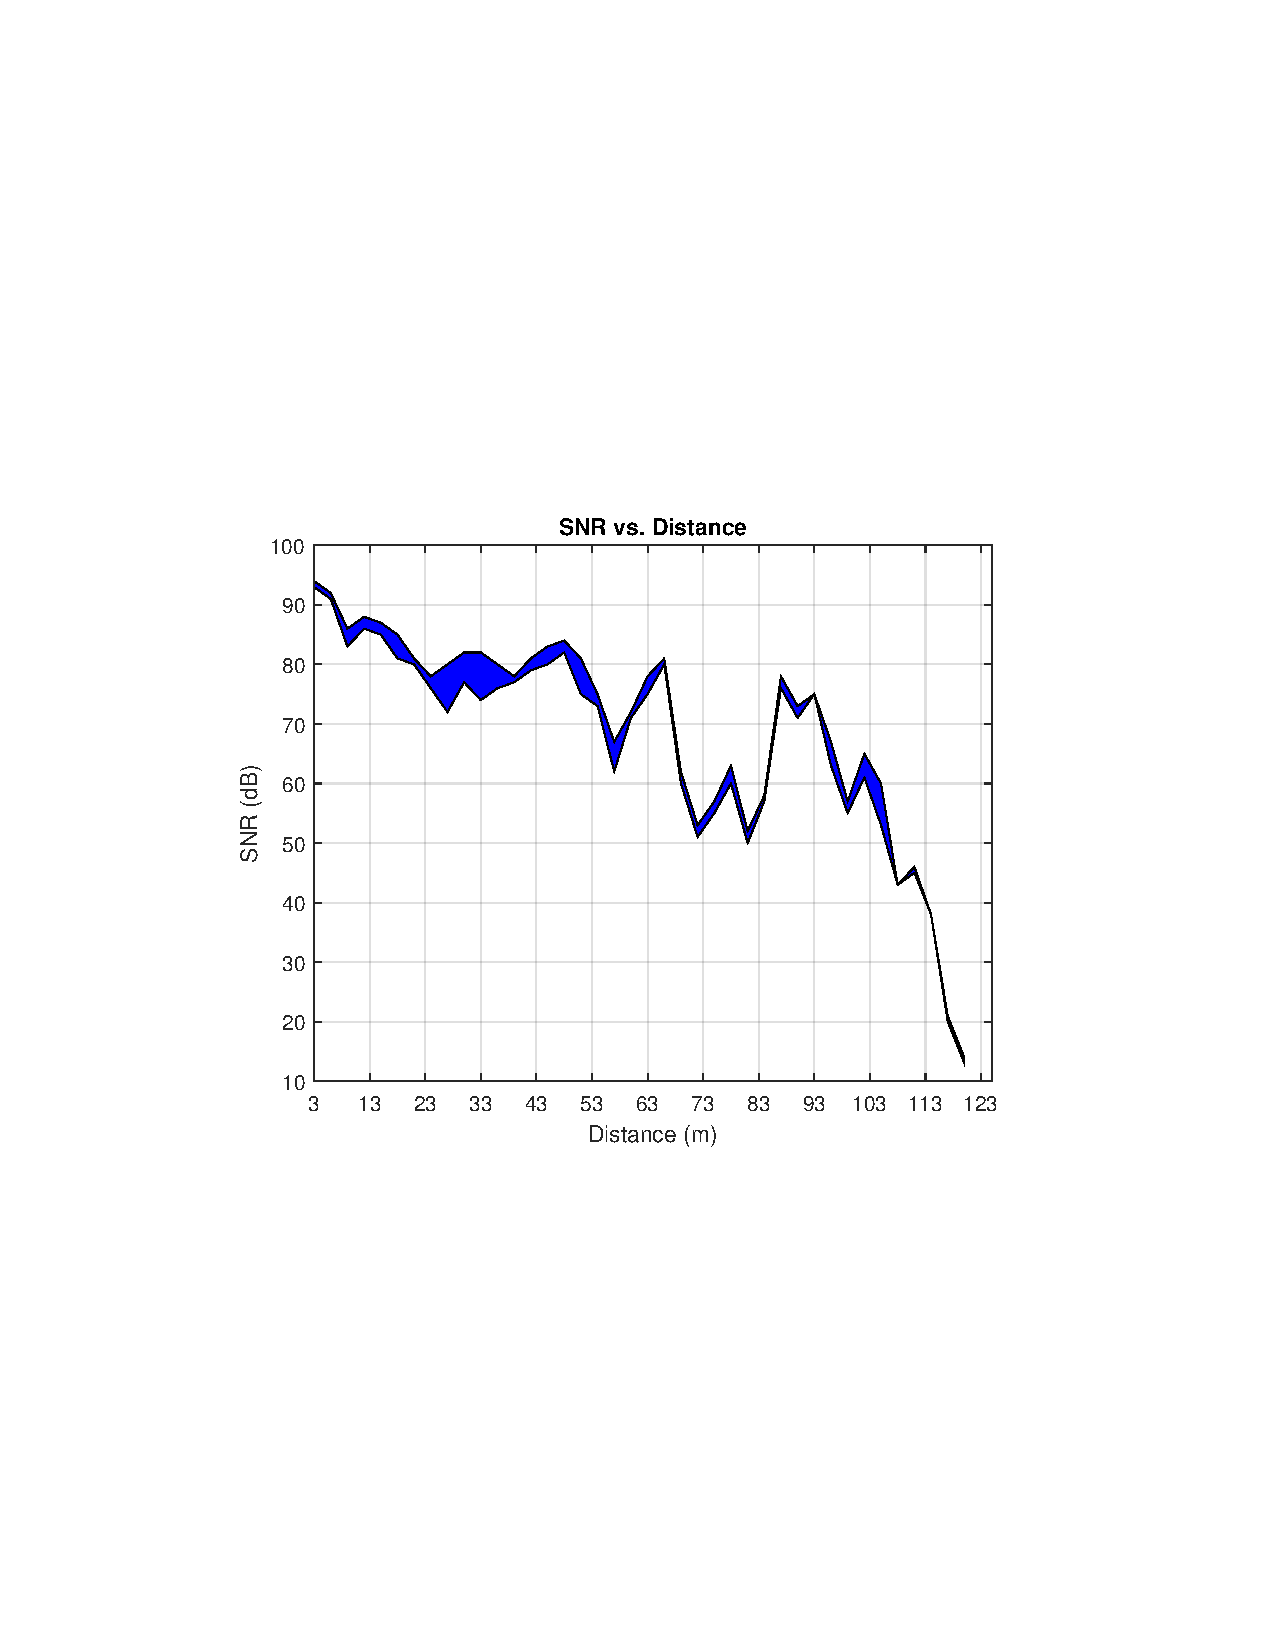
\includegraphics[width=5in]{snr}
	\caption{Average SNR vs Distance}
	\label{fig:snr-vs-distance}
\end{figure}

\subsubsection{Flying duration \& Batteries}

As shown in Fig.~\ref{fig:time-comparison} we have 
conducted time comparison experiments for both drone's
battery (2700mAh) and the Raspberry Pi battery (4000mAh) 
using different actions such as idle, hovering, 
moving forward, and moving backward. We repeated 
the same actions without video streaming so that 
we can see its effect on power consumption. 
All the batteries were charged fully, and the timer 
script stops when the battery percent reaches zero. 

First, as we predicted 
the maximum time reached is when both the drone and 
the Raspberry Pi are in an idle state, in which both case both will 
be on the ground without moving any motors.
This action still consumes energy but with 
its stability, over time ~\cite{Abey18}. 
The next action is when the drone is hovering, and 
the Raspberry Pi is sending navigation control 
signals to the drone and receiving video frames 
that are streamed to a web graphical interface. 
When the drone hovers without streaming, it worked 
for \SI{14.78}{minutes}, and when the camera is used for 
the stream which will add more power consumption to 
the drone battery; it worked for \SI{14.2}{minutes} which 
is less than the hovering without stream. The final 
action is when the drone takes off and keep moving 
forward, backward, left, and right, and in this action 
more energy consumption is seen and that made the 
battery for the drone survives only for \SI{13.58}{minutes}
when the camera is off, and for \SI{13.18}{minutes} 
when the camera and stream are on.

The main focus will be on the drone battery and every 
action energy. This is because the raspberry pi battery 
is not being highly affected by the actions. 
The next step is to derive the energy model for every 
action by using the distance and time. For the drone battery, 
we have 2700mAh which is 20.52Wh ~\cite{Par19}, 
we can get the drone energy by multiplying Wh by 3600 
so we will have a total of 73,872 Joules. When taking
hovering without stream as an example, the battery 
went from 100 percent to 0 in \SI{14.78}{minutes} which is 
886.8 seconds. We can say that the hovering action takes 
approximately 73,872/886.8 = 83.30 Joules/sec. 
For moving action,
we also considered the distance, so we kept 
moving the drone one meter in each direction 
{forward, backward, left, right} and then calculate 
the total distance traveled. The drone repeated 
the moving action 11 times, so the total distance 
is 44 meters and the energy per second consumed 
is 73,872/814.8 = 90.66 Joules/sec but this energy 
per second is for the 44 meters, so we can get the 
energy per second for 1 meter by calculating 
90.66/44 = 2.06 Joules/s. 
In (\ref{eq:Energy-moving}) we can generalize an energy 
equation for moving action, which can be used in the simulation 
environment to train the RL model. Now the model will not 
just consider the time, but also the energy consumption.
We verified the flight duration constraint, and we can devise some 
realistic energy models, that can be fed in the simulation 
to do the comparisons. This will help the RL model to choose 
the best action depending on less energy consumption 
when both actions have the same probability. 

\begin{align}
	P = \frac{E(J)}{t(s)} 
	\label{eq:power}
\end{align}

\begin{align}
	E = 2.06t*d
	\label{eq:Energy-moving}
\end{align}

\begin{figure}[!t]
	\centering
	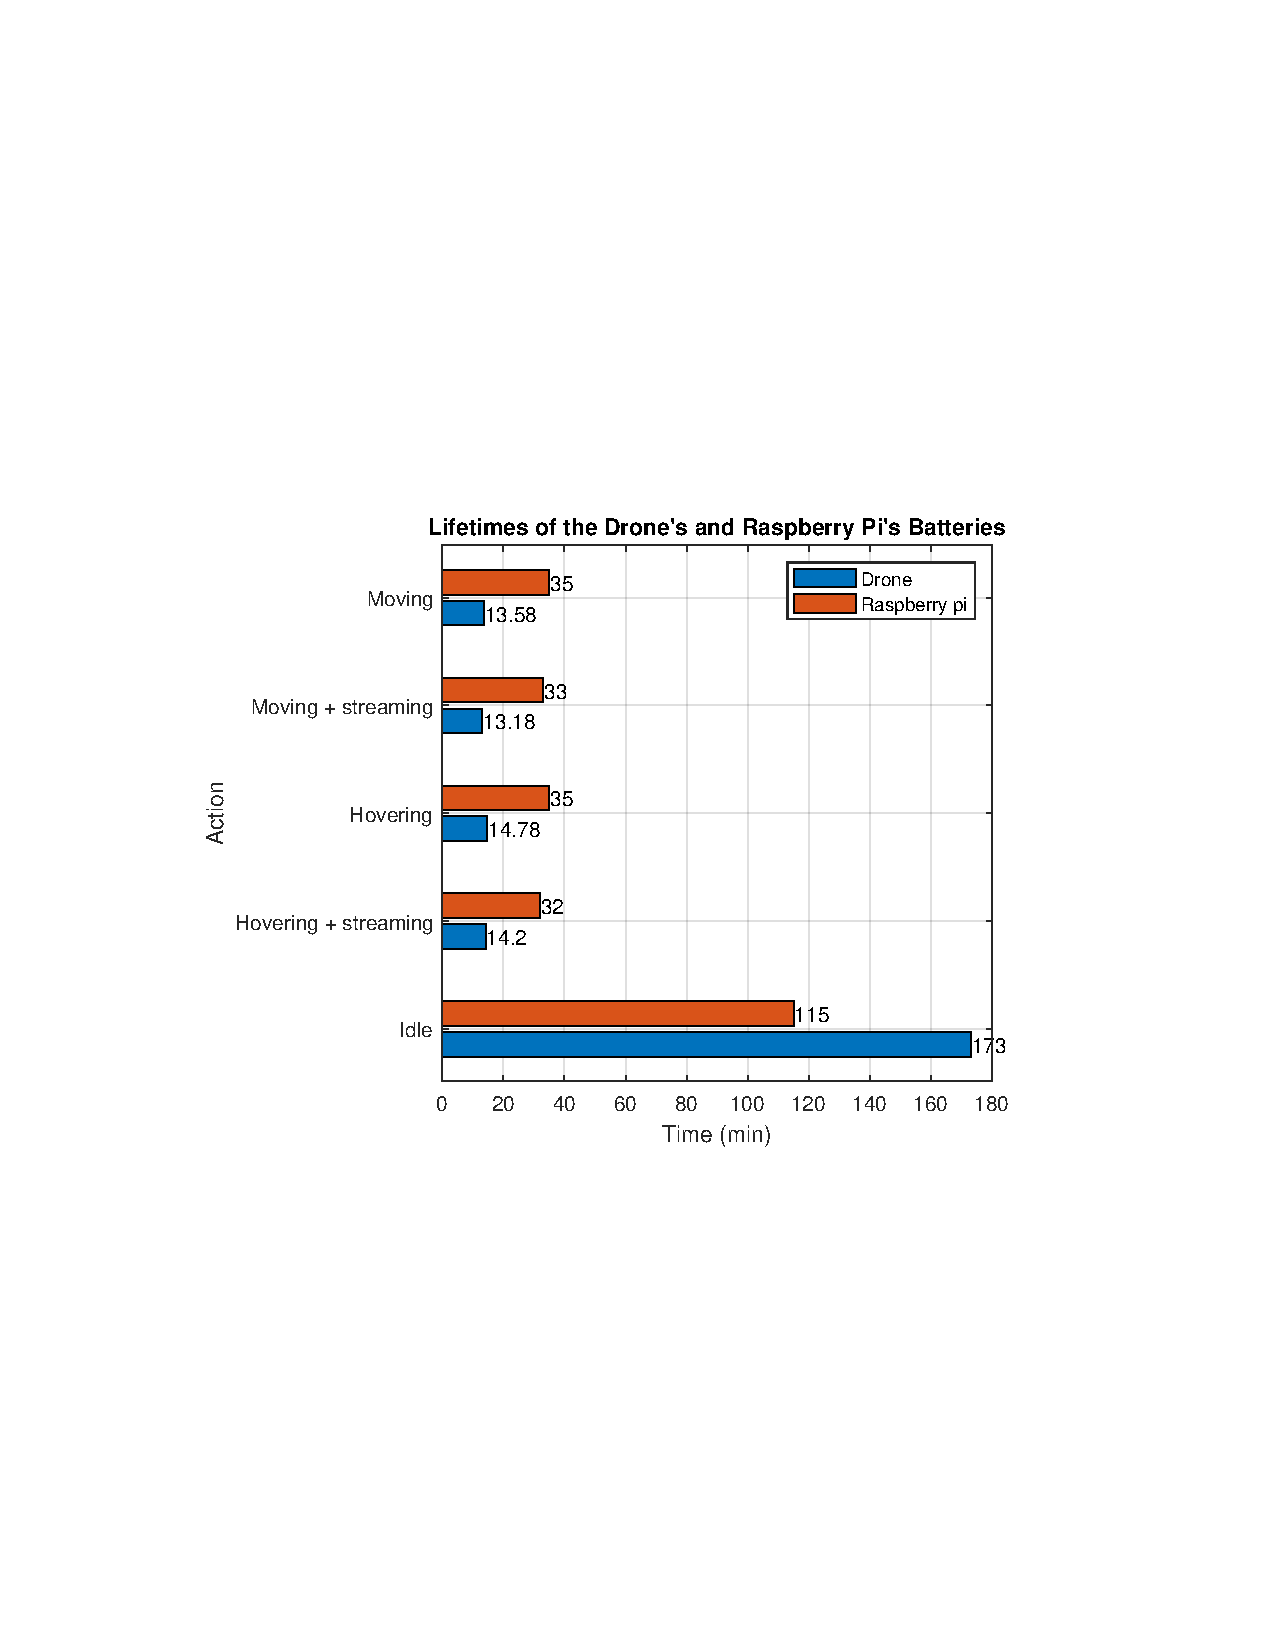
\includegraphics[width=5in]{battries-time}
	\caption{Battery's lifetime comparison.}
	\label{fig:time-comparison}
\end{figure}

\subsubsection{Response time}

We have done another experiment regarding the response time 
of the drone after sending a command to it from the Raspberry Pi. 
Calculating the response time was by starting a timer when 
sending the command and stopping it when the 
state of the drone changes. 
The experiment was done on simulation using Sphinx,
then we moved to the real world using the \anafi drone.
From \cref{tab:respone-time}, 
we can see that all the results are less than \SI{1}{second}
which satisfied our response time constraint.
Another point we can conclude from the table is that 
the response time of the real world is less than 
the simulation, and this is predictable since the simulation
depends on the \textsc{gpu} power and processing time. 

\begin{table}[H]
	\centering
	\caption{The average response time of the drone after sending a control command.}
	\label{tab:respone-time}
	\begin{tabularx}{0.7\textwidth}{ X c c }
		\toprule
		\textit{} & \textit{Simulation} & \textit{Real-world}\\ \midrule
		Motor ramping for takeoff (seconds)  & 0.3506 & 0.0323     \\
		Move while flying (seconds) & 0.7441  & 0.1511   \\
		\bottomrule
	\end{tabularx}
\end{table} 

\subsubsection{Payload}

As shown in \cref{fig:payload}
we attached \SI{180}{grams} of Raspberry Pi and Arduino boards
to see the effect on the performance, flight and
battery drain percentage. 
The drone has taken off successfully, 
but it was struggling to move, and we faced an expected 
battery drain that went from 
\SI{100}{\percent} to \SI{90}{\percent} in 
\SI{1.5}{minutes}. This is because the propeller motors will try to push 
their limits to take off the drone, which will consume more energy.
After adding payload to the drone at \SI{200}{grams}, the drone could not
takeoff, and we now know the payload limit for the takeoff. 
We noticed that the drone movement
is not normal when the payload exceeds \SI{180}{grams} 
so we considered that and changed
the payload constraint. In the actual design, as shown in 
\cref{fig:actual-total-weight} the total payload 
is \SI{193}{grams} which is more than the payload constraint. 
The drone movement was bad, so we removed the 3D printed
parts to reduce the weight to \SI{172}{grams}, 
which makes the movement now smooth and stable.



\begin{figure}[H]
	\centering
	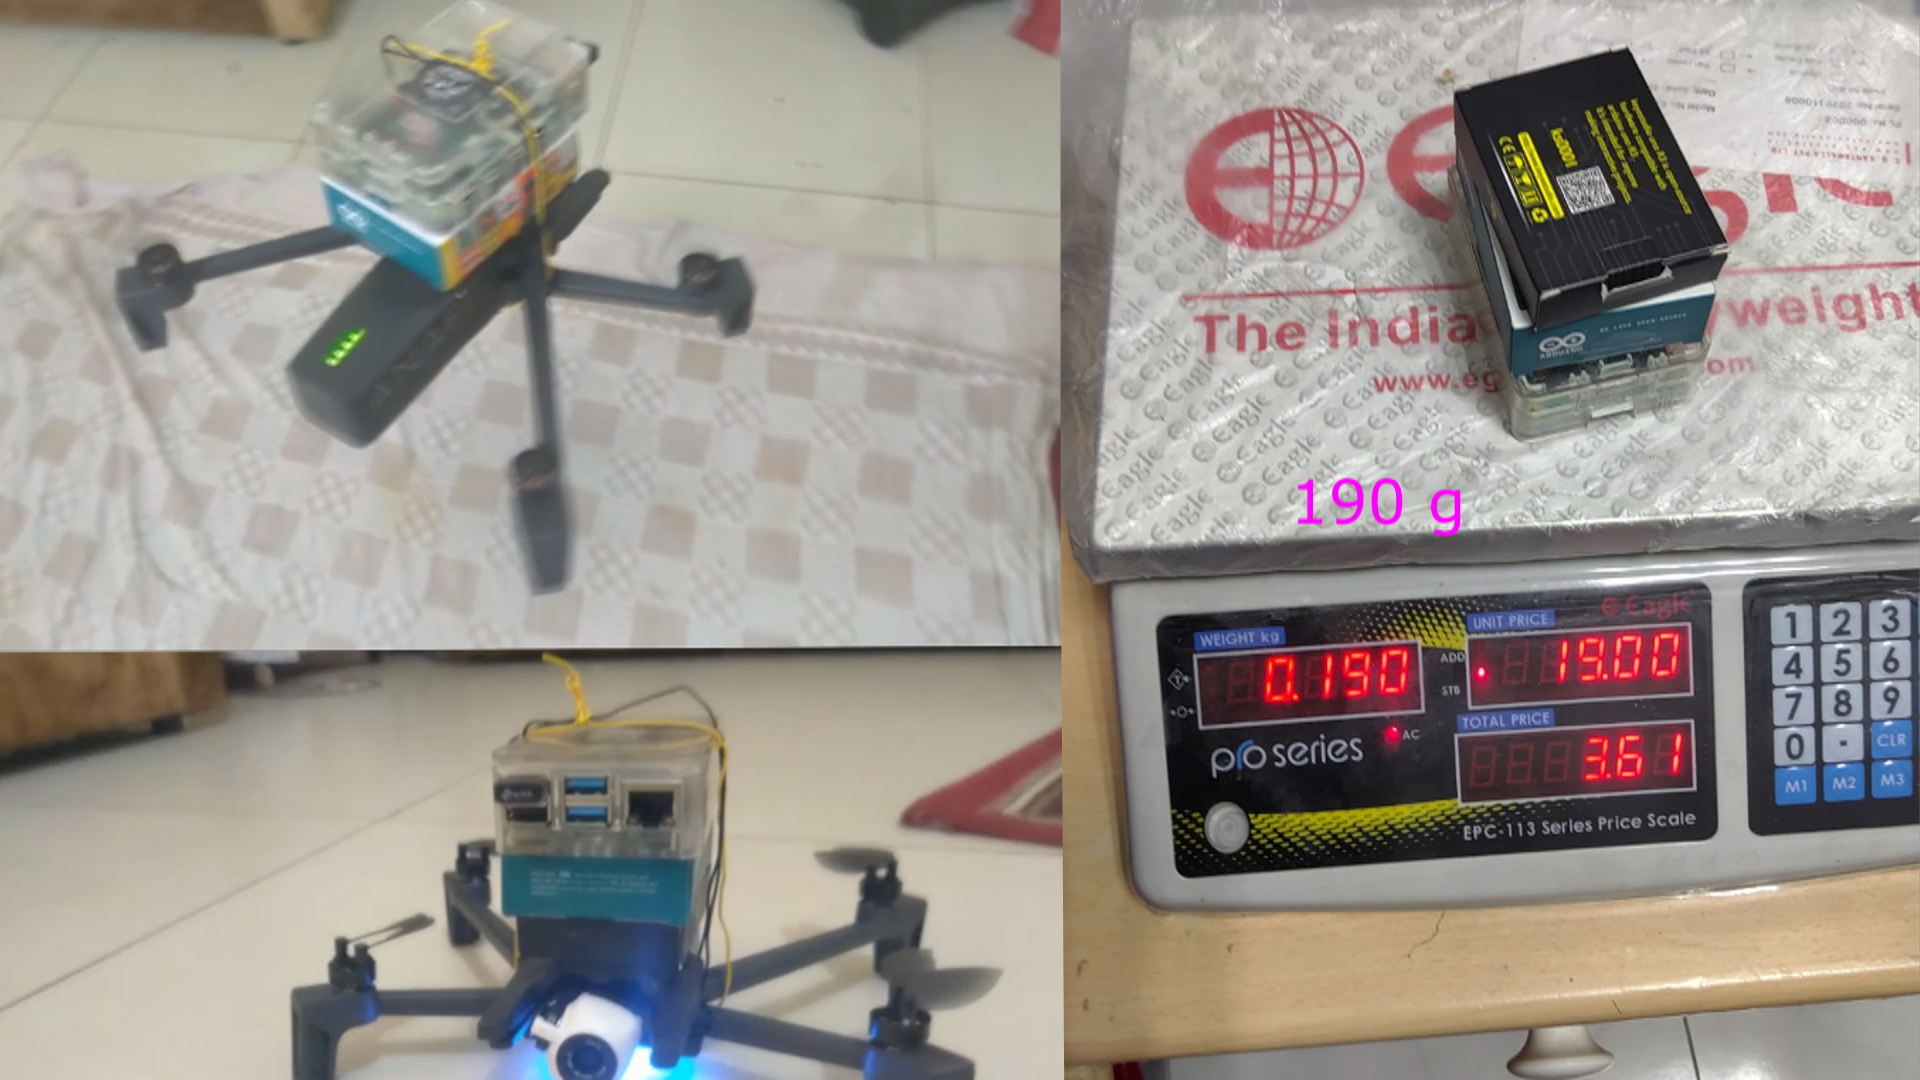
\includegraphics[width=0.6\textwidth]{payload.png}
	\caption{The total weight of test payload}
	\label{fig:payload}
\end{figure} 

\begin{figure}[H]
	\centering
	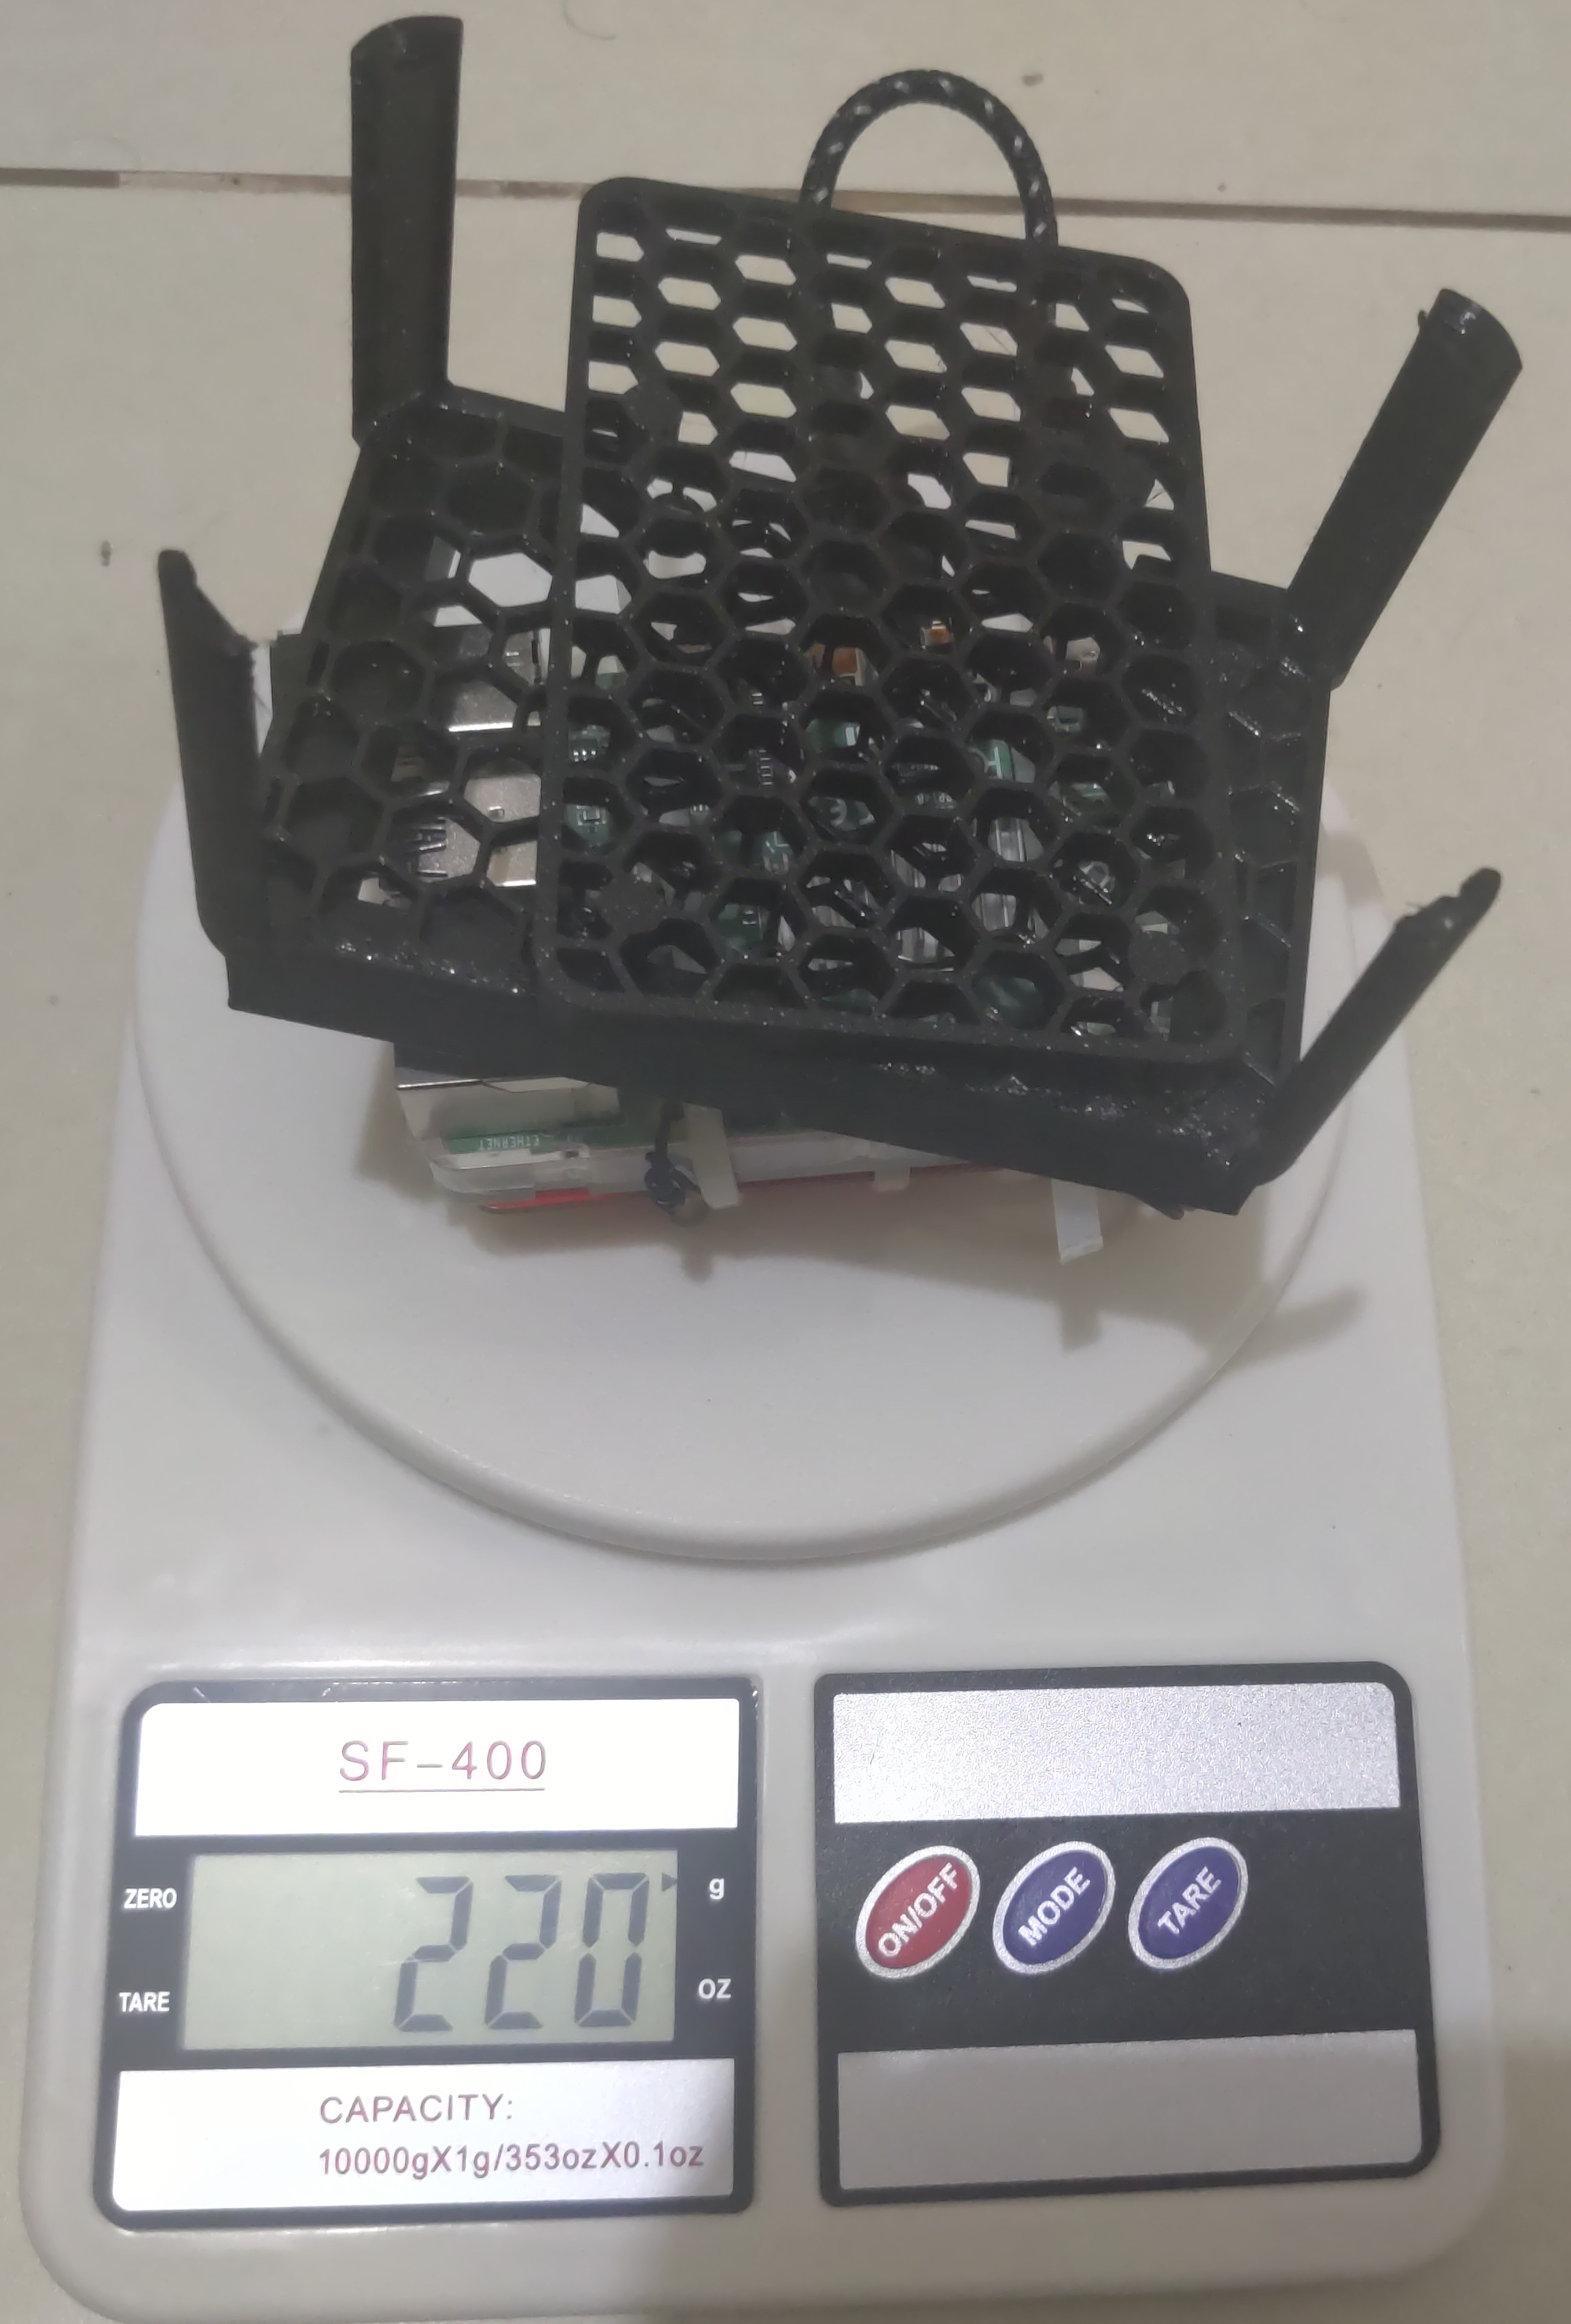
\includegraphics[width=0.4\textwidth]{totalweight.jpg}
	\caption{The total weight of actual payload}
	\label{fig:actual-total-weight}
\end{figure} 

\subsection{Integration testing}
This section will discuss the results of the 
real-world experiments, the challenges we have faced,
and how we resolved them.
\subsubsection{Environment}
Finding the best location for testing was difficult
because our requirements depend on multiple factors 
such as \gls{gps} signal, free space, dimensions,
and flying drones regulations. After multiple investigations
at different locations, as shown in \cref{fig:testing-location}
we have found that the QU football court was an optimal location
for testing, since there is good \gls{gps} coverage and the dimensions are
enough for our testing. In addition, the fence was high enough so that
the drone cannot exceed the local property flying limit.
We have set up the \textsc{qr} codes, drone, on-board computer, 
and the command-control
system laptop to start testing three experiments in the section below.

\begin{figure}[H]
	\centering
	\includegraphics[width=0.9\textwidth]{location.jpg}
	\caption{Environment location \& the setup}
	\label{fig:testing-location}
\end{figure} 
\subsubsection{Movement and detection}
In this experiment, we want to verify that drone movement, and
\textsc{qr} codes detection works perfectly. This experiment is 
essential since it is the building block for coming experiments
that need those two primary functions to be fully functional.

We have started the mission from the command and control system, 
the on-board computer responded and sent the control commands 
to the drone shown in \cref{fig:experiment-drone}.
The drone moved to the cells without any issues,
and the detection tool started to analyze 
the video feed to detect the \textsc{qr} codes.

The results, as shown in \cref{fig:detection-camera}, 
the detection tool detected all the targets correctly 
without any missing targets. Also, some challenges 
in the movement have been resolved and listed in 
the challenges table. By now, we are ready to do the main tests.

\begin{figure}[H]
	\centering
	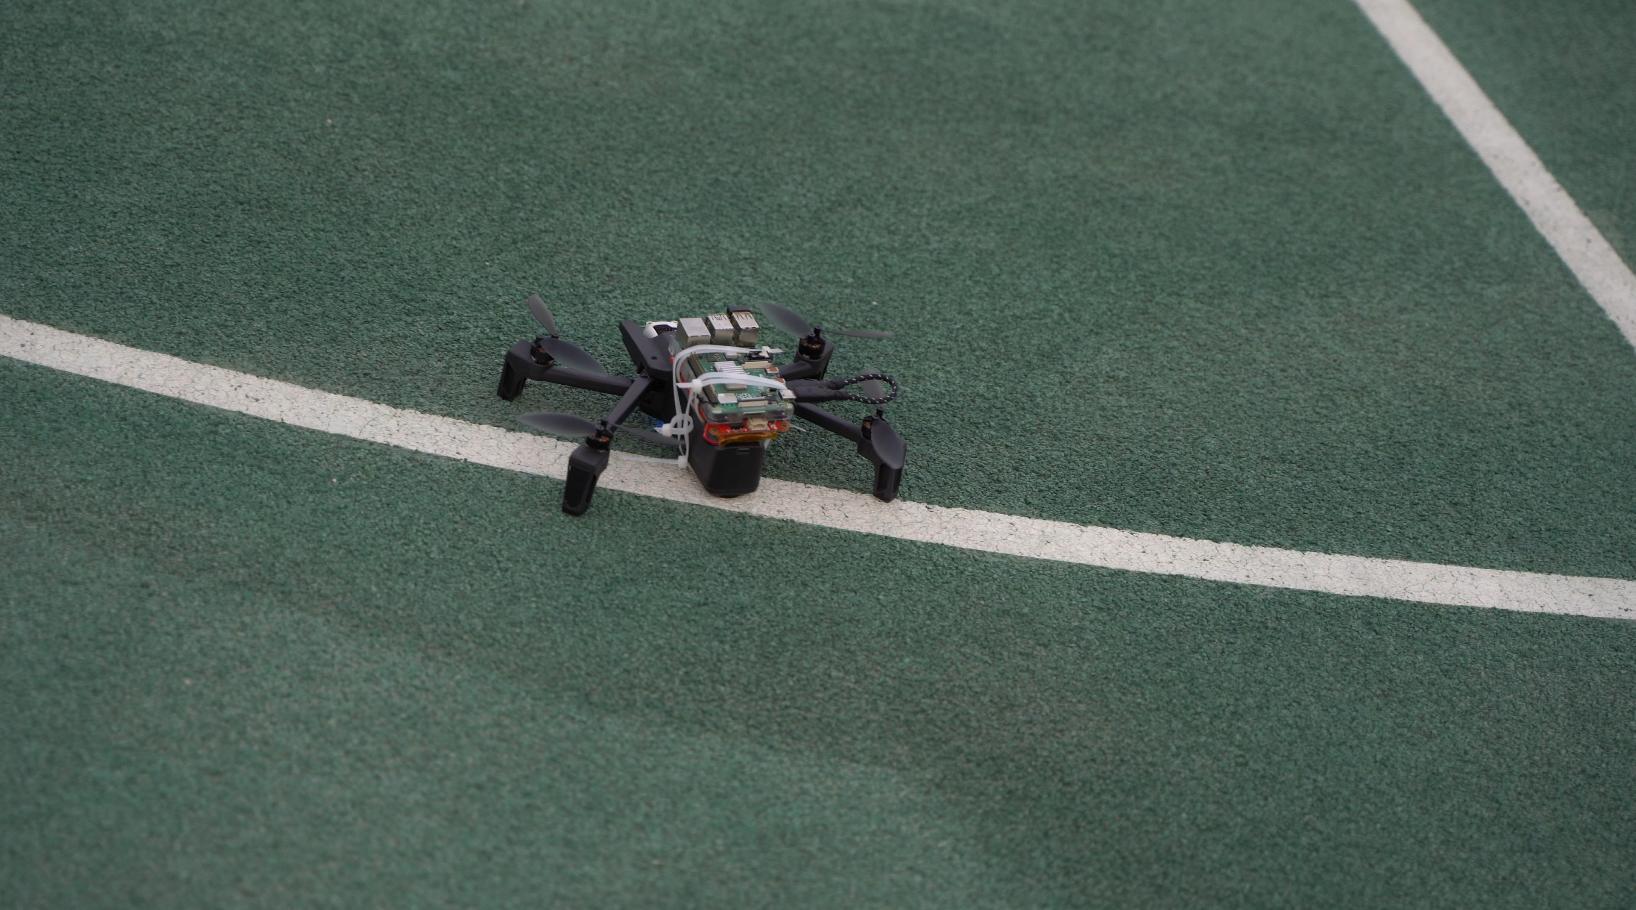
\includegraphics[width=0.7\textwidth]{drone.png}
	\caption{Drone setup used}
	\label{fig:experiment-drone}
\end{figure} 

\begin{figure}[H]
	\centering
	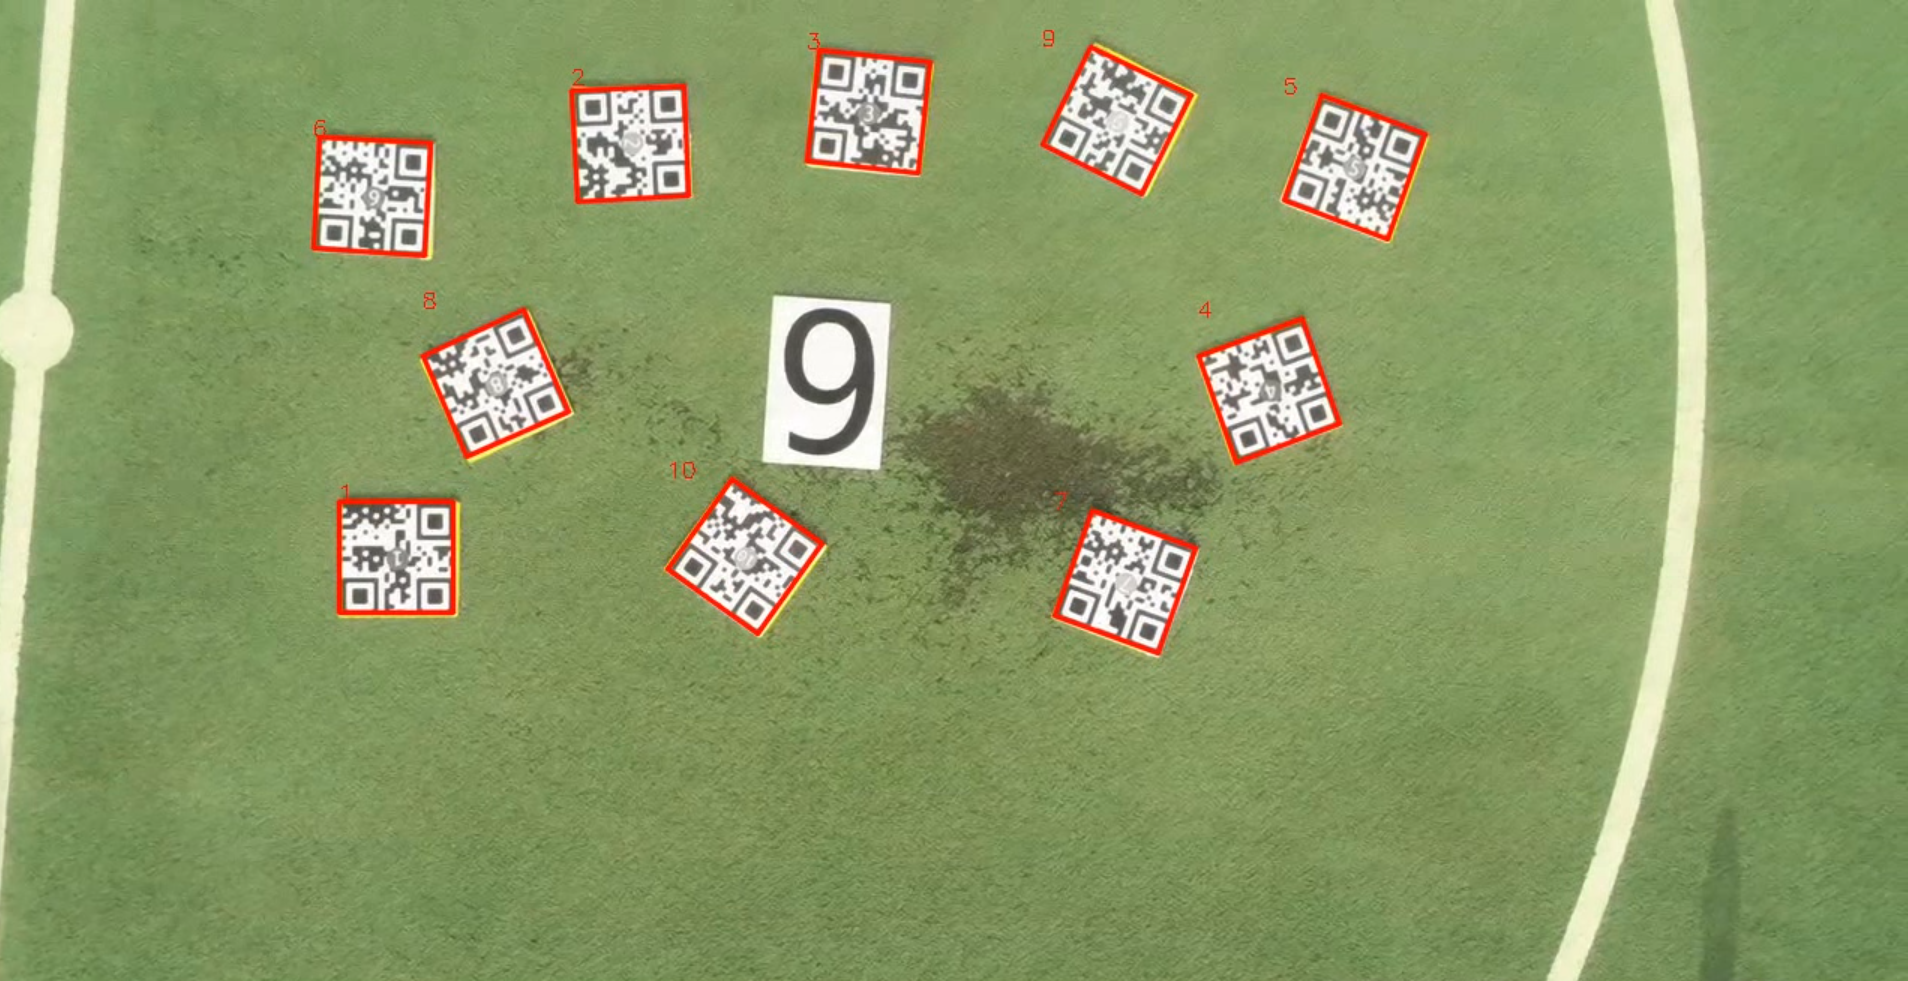
\includegraphics[width=0.7\textwidth]{detection-camera.png}
	\caption{Detection results}
	\label{fig:detection-camera}
\end{figure}

\subsubsection{Fixed targets}
In this experiment, we have tested the drone fixed targets
visitation task, we have tried to keep the environment similar
to the simulation environment to verify the digital twin technology.
Firstly, as shown in \cref{fig:targets-location},
we have distributed the \textsc{qr} codes at southeast cells 
{19,20,24,25} ,this is because we are following 
the same normal distribution that has been used in the simulation.

We have started the mission, in \cref{fig:fixed-location-detection-camera}
the drone did the whole mission in five steps by going
to the southeast cells and detecting the unique targets. 
The drone did not detect one target in 
step two (cell 25), so it returned to it in step five. Finally,
since the drone covered all the targets, it 
went to land at the original takeoff cell.

The whole mission took \SI{35}{seconds} to cover all the targets,
which is a good number compared to other techniques such as zigzag.

\begin{figure}[H]
	\centering
	\includegraphics[width=0.8\textwidth]{drone-fixed.png}
	\caption{The setup for the fixed targets}
	\label{fig:targets-location}
\end{figure}


\begin{figure}[H]
	\centering
	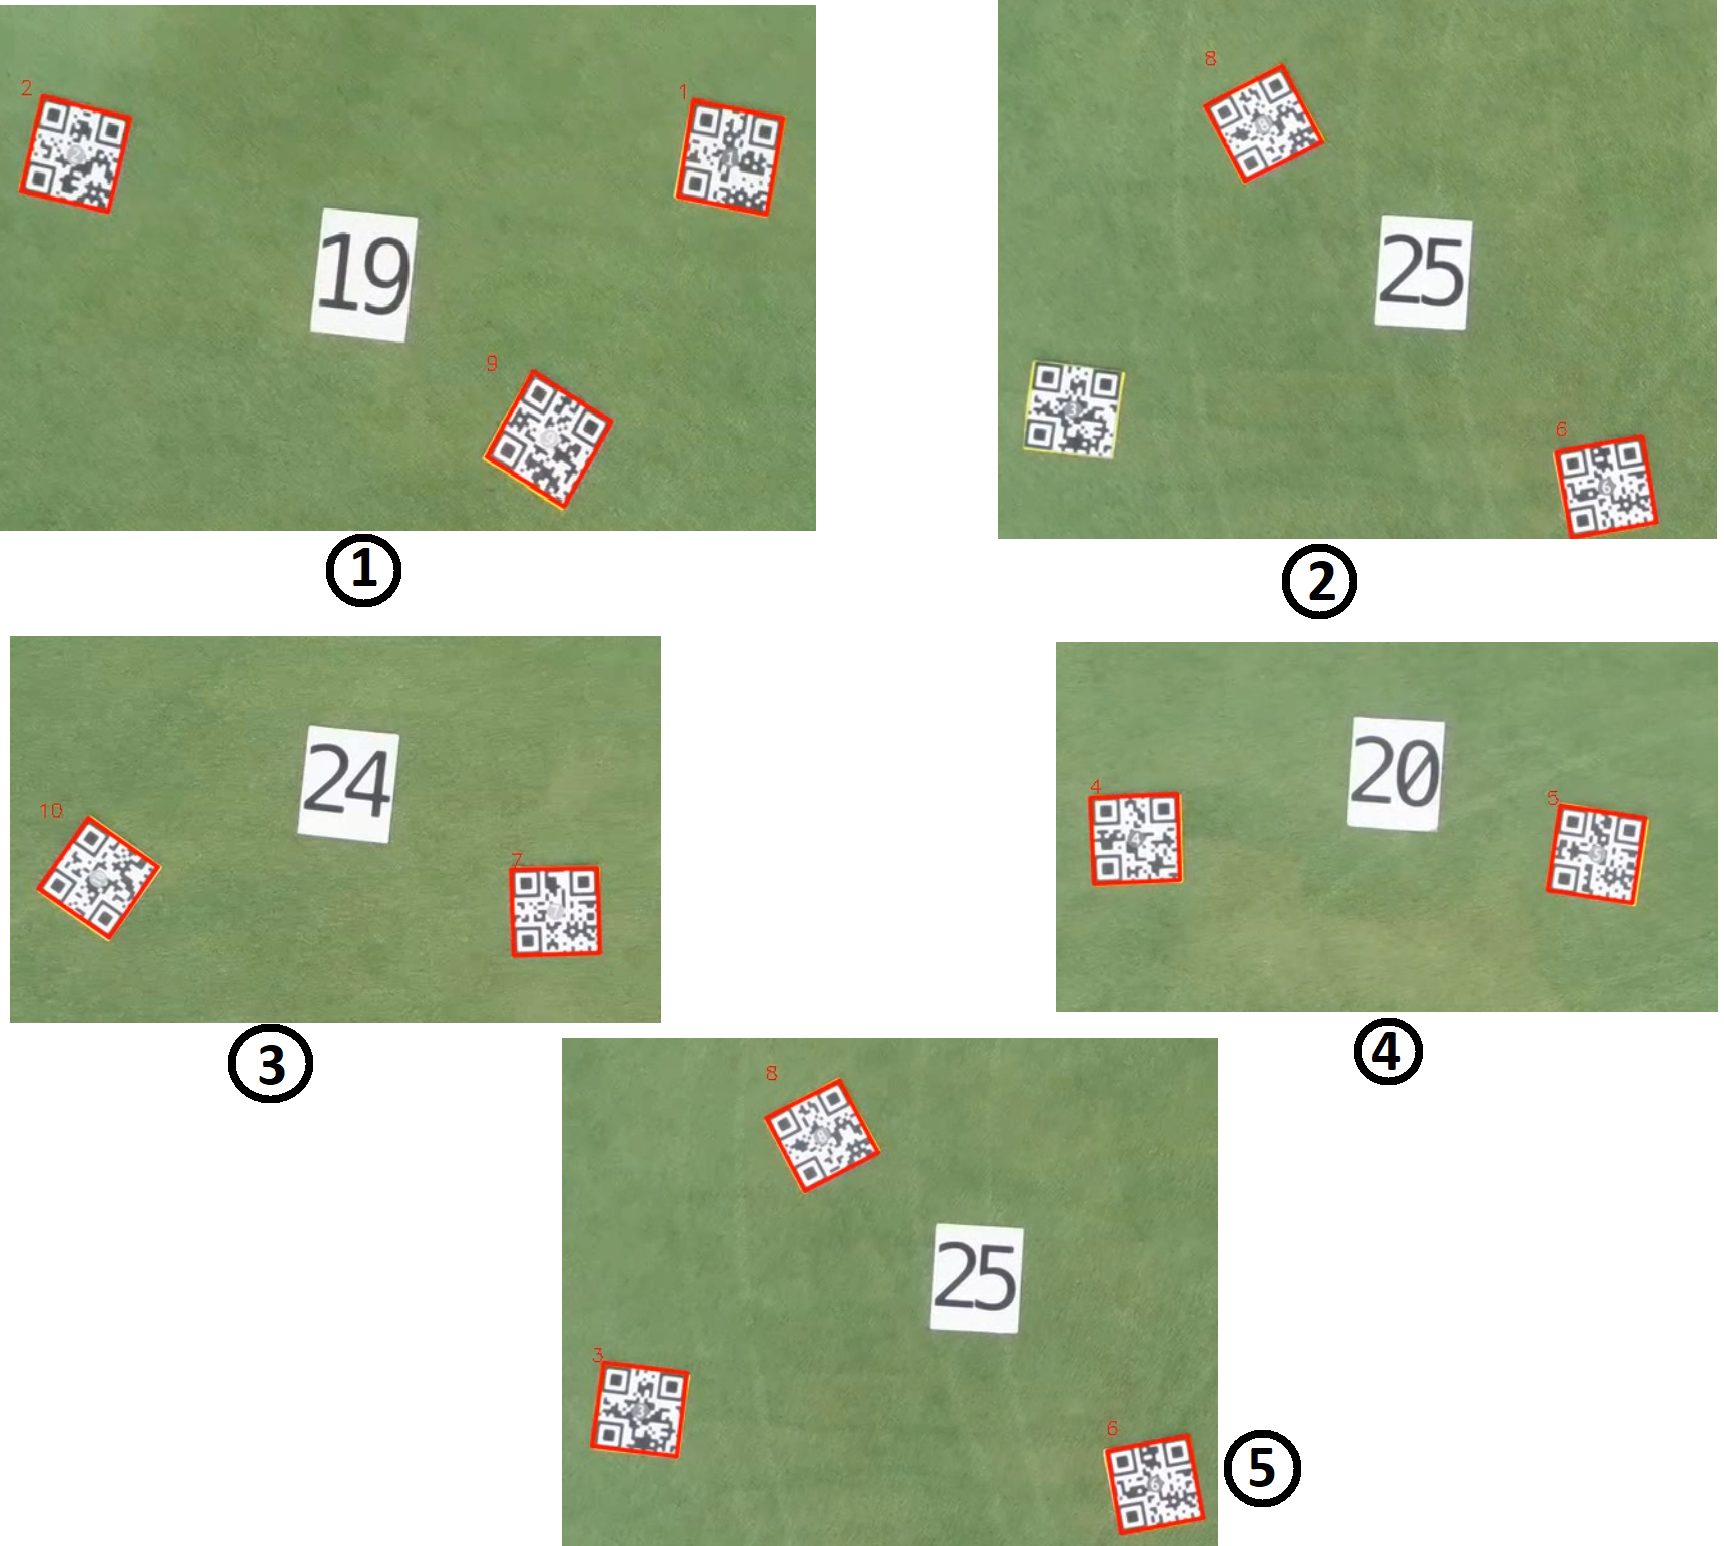
\includegraphics[width=1\textwidth]{fixed-targets-detection.png}
	\caption{Fixed targets visitation results}
	\label{fig:fixed-location-detection-camera}
\end{figure}


\subsubsection{Moving \& fixed targets}
The last experiment will have both fixed and mobile targets,
again we will try to make the environment the similar to the 
simulation, so for moving targets as shown in 
\cref{fig:mobile-targets-real-experiment}, we will have 
three programmed Lego EV3 that will start 
from the south and will go 70\% of the time to the north-west 
and the 30\% of the time to random remaining direction. For fixed
targets they will be distributed according to the generated distribution
as shown before in \cref{fig:fixed-position-distribution}.

Firstly, the drone will go to cover all the fixed targets, and one of the 
results is shown in \cref{fig:fixed-mobile-expriment}. After the 
drone finished all fixed targets, it went to the mobile targets cells and
started to detect them. The result in \cref{fig:fixed-mobile-expriment} 
shows that it detected all the mobile \& fixed targets, 
then it went to landing since it covered all the fixed and mobile targets.
There are some challenges in the movement of the robots, which are 
discussed in the challenges table.


\begin{figure}[H]
	\centering
	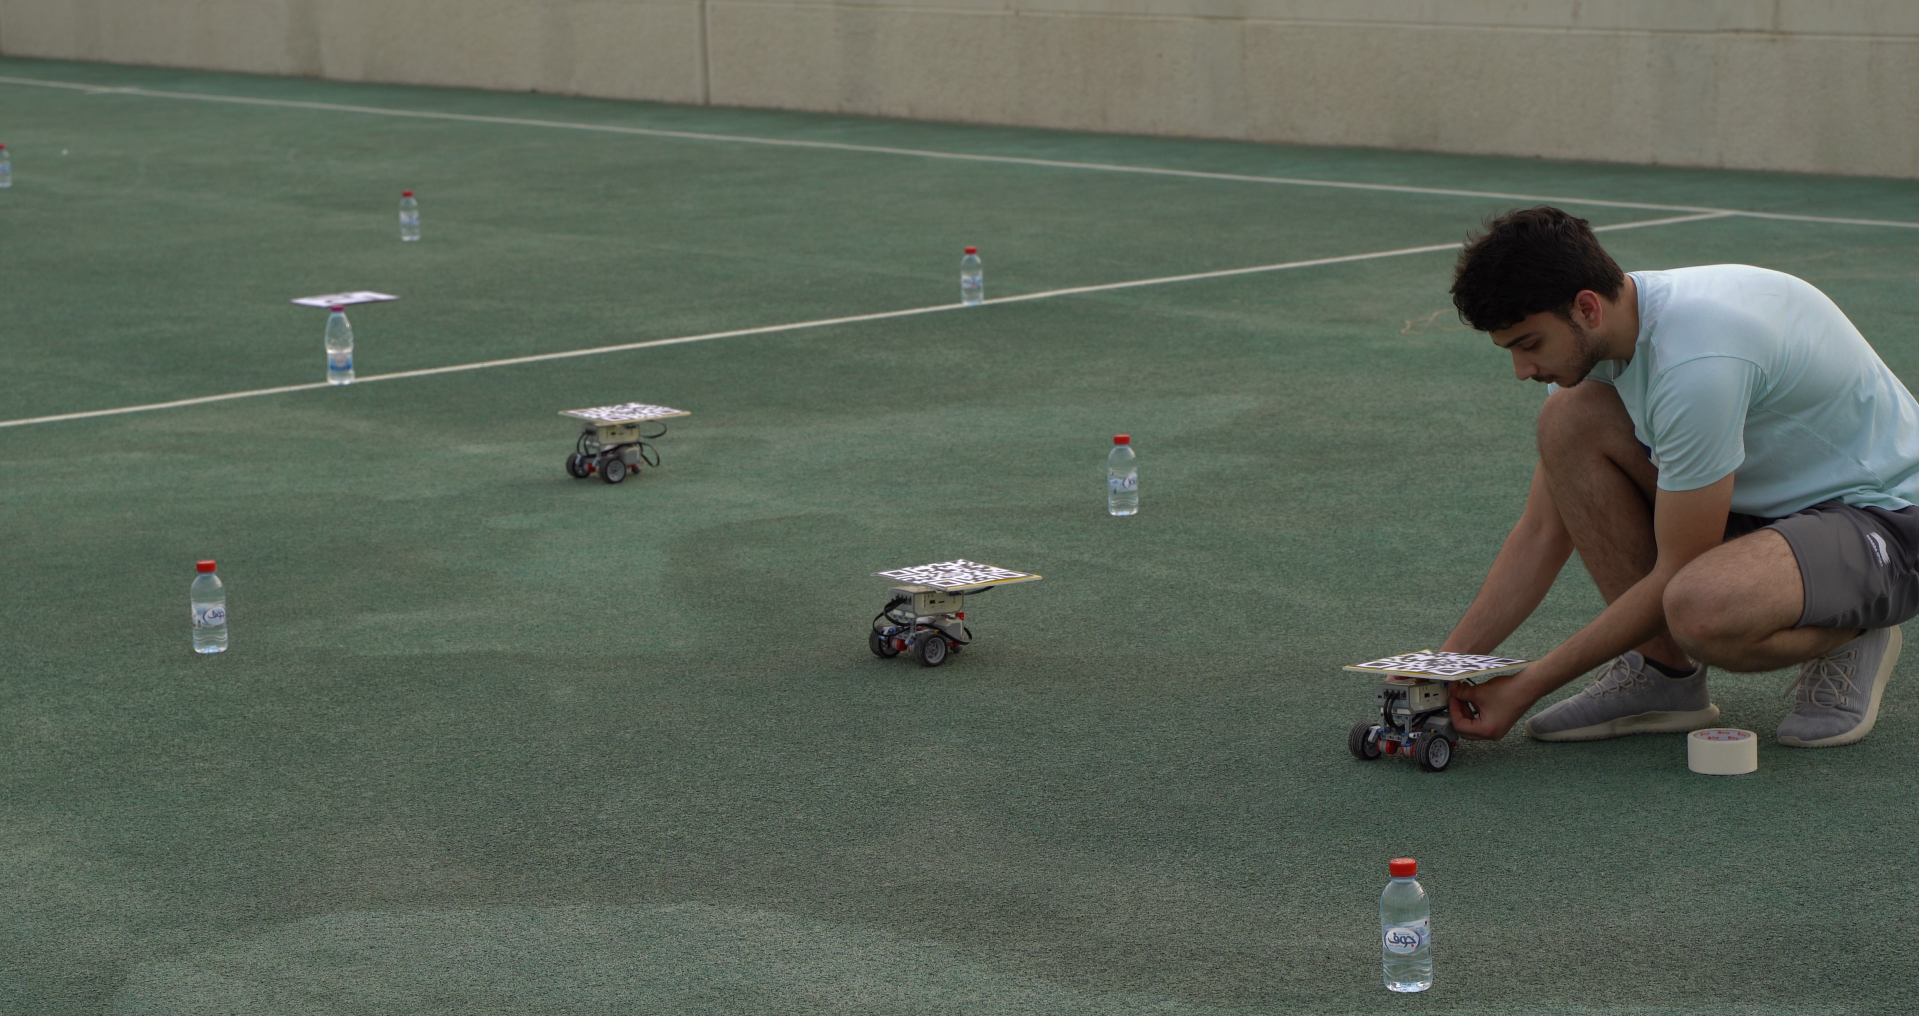
\includegraphics[width=0.8\textwidth]{mobile-targets-real-experiment.png}
	\caption{The setup for the mobile targets}
	\label{fig:mobile-targets-real-experiment}
\end{figure}

\begin{figure}[H]
	\centering
	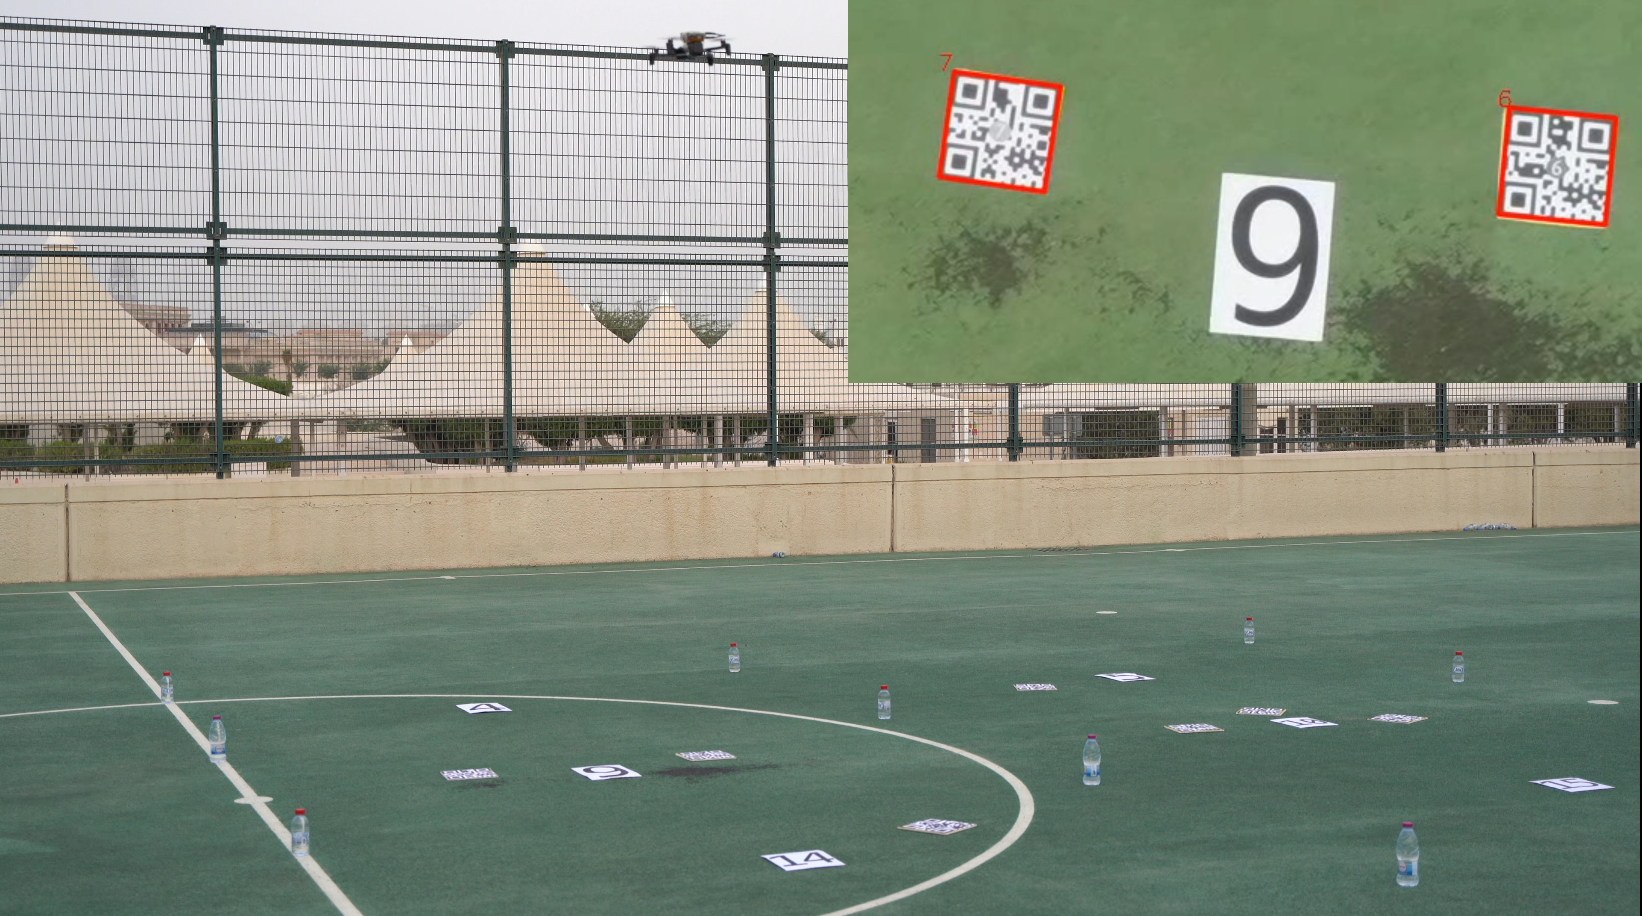
\includegraphics[width=0.8\textwidth]{fixed-mobile-expriment.png}
	\caption{The results of the fixed-targets}
	\label{fig:fixed-mobile-expriment}
\end{figure}

\begin{figure}[H]
	\centering
	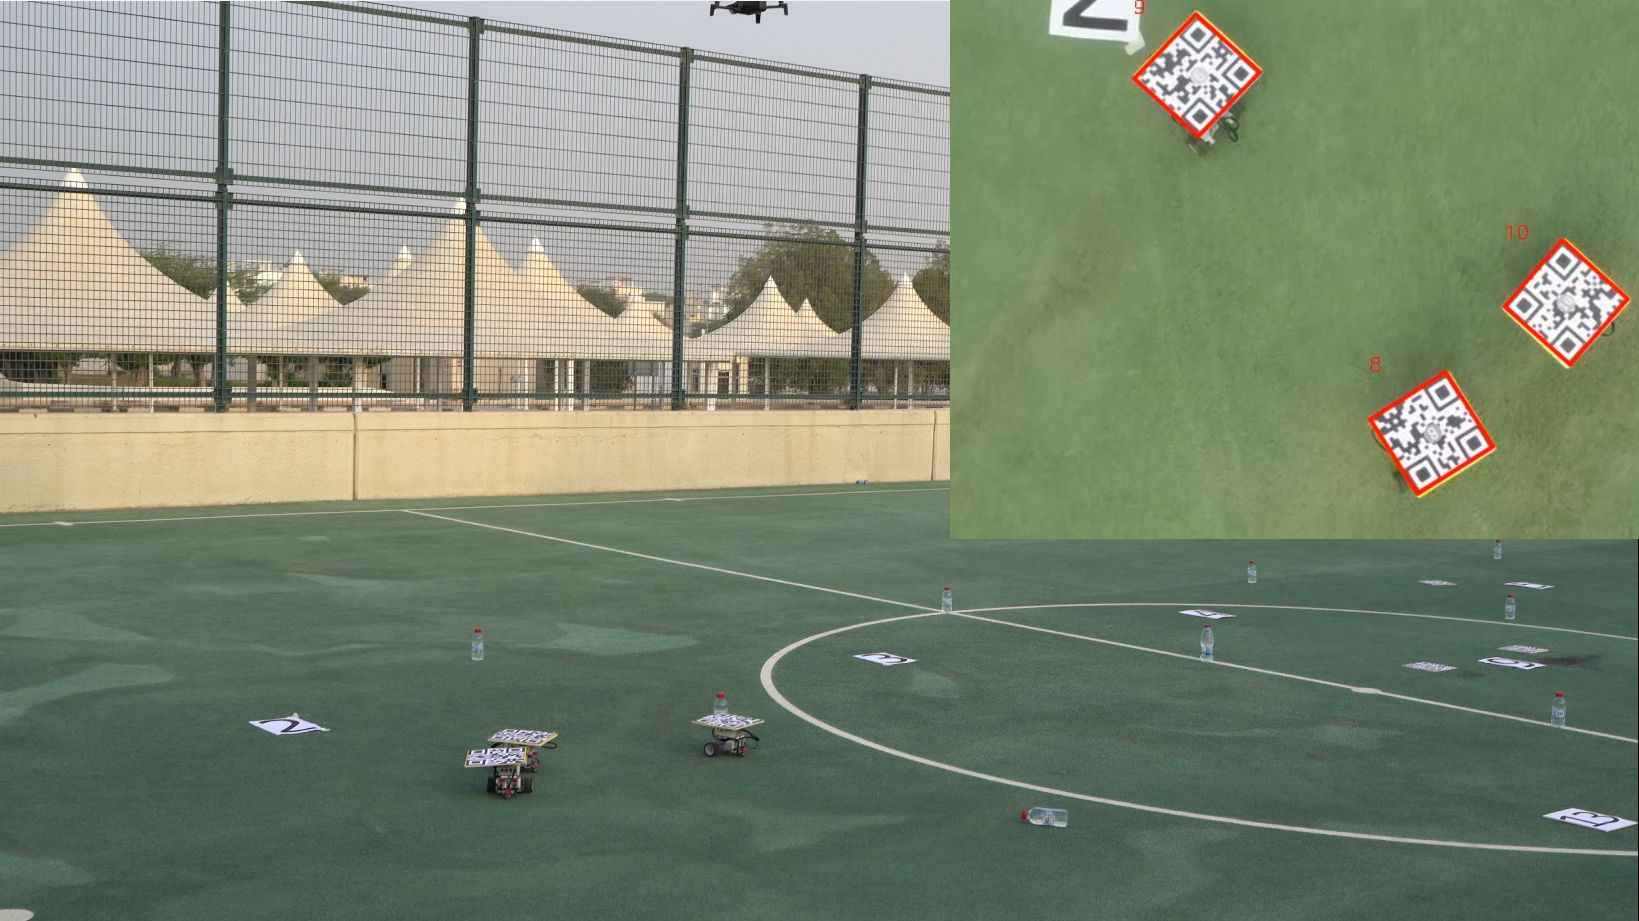
\includegraphics[width=0.8\textwidth]{mobile-targets-detection.png}
	\caption{The results of the mobile-targets}
	\label{fig:mobile-expriment-detection}
\end{figure}

% SOFTWARE
\subsection{\textsc{rl} training}

\begin{table}[H]
    \centering
    \caption{Summary of the \gls{rl} and simulation testing}
    \label{tab:rl-testing-summary}
    \begin{tabularx}{\textwidth}{ X X l X l }
        \toprule
        \textit{Constraint} 
            & \textit{Testing procedure} 
                & \textit{Result}
        & \textit{Measurement data} 
            & \textit{Error (\%)} \\

        \midrule
        
        
        \raggedright Training convergence    
            & Train the agent until the episode rewards converge to a
            value
        & Met
        & Episode rewards converged to around 13 and 8 (for fixed-targets training
        and mobile-targets training respectively)
        & N/A \\
        \addlinespace

        \raggedright Model performance
        & Compare the \gls{rl} agent with random and zig-zag agents
        & Met
        & The \gls{rl} agent performed much better in terms of time
        and energy for fixed-targets and mobile-targets missions
        & N/A \\
        \addlinespace

        \raggedright Drone's height vs. cell width
        & Fly the drone at different heights and record the maximum
        width that it is able to cover
        & Met
        & The regression line manages to fit all point with a
        Pearson's $r$ value of 0.999958
        & 
        \begin{tabular}{l}
            \\
            $1-r^2 =$ \\
            $8.32\times 10^{-3}$ \\
        \end{tabular}
        \\
        % $1-r^2$ \newline $= 8.32\times 10^{-3}$ \\
        \addlinespace

        \bottomrule		
    \end{tabularx}
\end{table}

\subsubsection{Fixed-targets mission}

After 50,000 timesteps of training using the Proximal Policy
Optimization (PPO) algorithm, the average episode reward converged
to around 13 as shown in \cref{fig:episode-rewards-fixed}.
The agent did not achieve the maximum return of 15
on average
due to several reasons. Firstly, the
targets kept changing positions from episode to episode.
Secondly, the softmax output layer of the PPO still produced 
a healthy amount
of exploration away from the targets in some episodes,
and finally, the imperfection in the object detection model made
the agent unable to collect the reward it has received. 
% thinks it moved to a wrong cell when it actually
% did not.
% The Pyzbar library used for object detection has
% an accuracy of up to 90\% in good conditions, but it can 
% be as low as 30\% when the QR code is damaged due to
% an error in photo capturing and processing~\cite{dynamsoft}.

\begin{figure}[!t]
	\centering
	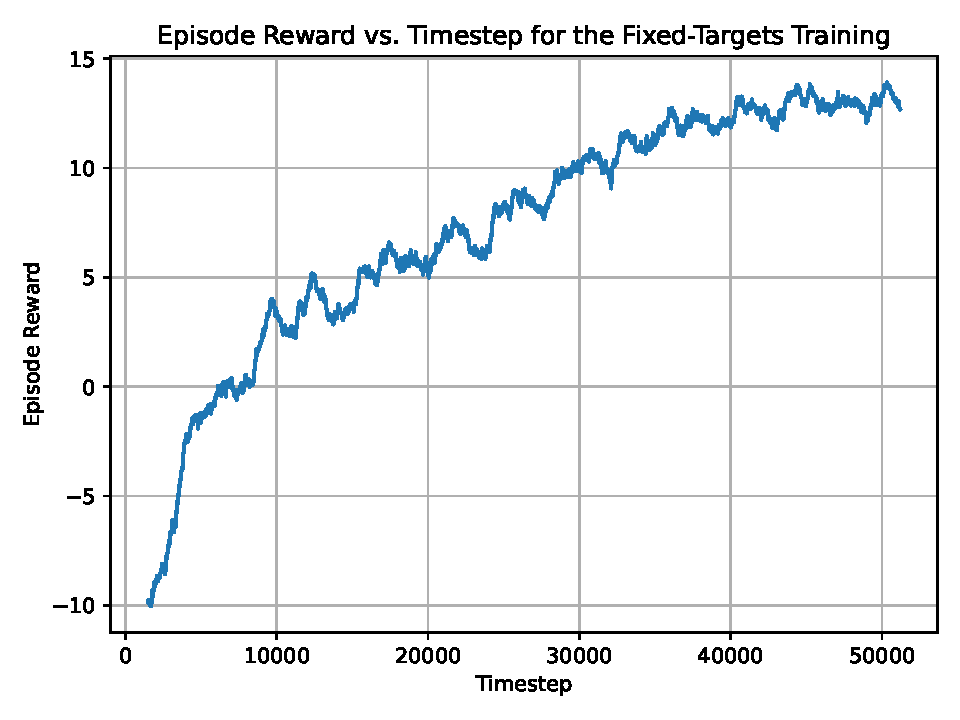
\includegraphics[width=0.8\textwidth]{episode-rewards-fixed}
        \caption{\gls{rl} episode reward convergence during the
        fixed-targets training.}
        \label{fig:episode-rewards-fixed}
\end{figure}

Similarly, \cref{fig:episode-lengths-fixed} shows the the number of
timesteps the agent performed before accomplishing the mission
(visiting all targets) in each episode.
The succesful learning can also be observed here where the agent took
fewer and fewer timesteps as the training was progressing.
It starts at the maximum allowable timestep of 15 and converges at
around 5.

\begin{figure}[!t]
	\centering
	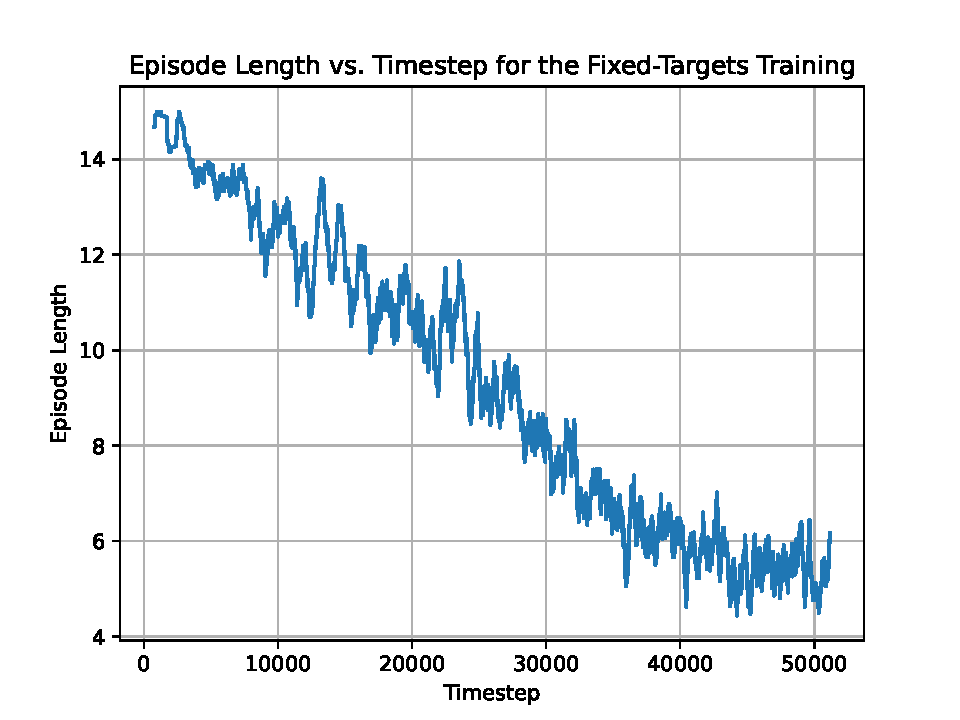
\includegraphics[width=0.8\textwidth]{episode-lengths-fixed}
        \caption{\gls{rl} episode length convergence during the
        fixed-targets training.}
        \label{fig:episode-lengths-fixed}
\end{figure}

\subsubsection{Mobile-targets mission}

As explained in the \cref{sec:implementation}, in this type of
mission, three targets are mobile while the rest are stationary.
The training for this took 100,000 timesteps to achieve conversion as
shown in \cref{fig:episode-rewards-mobile}.
The converged value is around 8, much lower than the static-targets
mission.
This is because the three moving targets added much more complexity in the
learning.

\begin{figure}[!t]
	\centering
	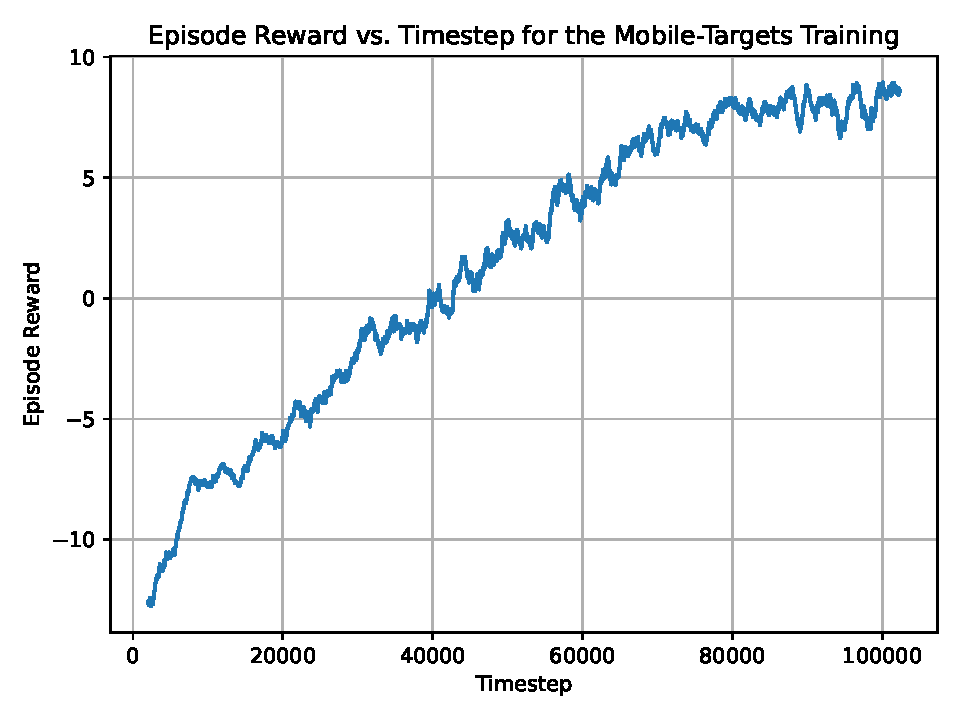
\includegraphics[width=0.8\textwidth]{episode-rewards-mobile}
        \caption{\gls{rl} episode reward convergence during the
        mobile-targets training.}
        \label{fig:episode-rewards-mobile}
\end{figure}

The same trend as the static-targets mission can also be seen in
\cref{fig:episode-lengths-mobile}.
The differences lie in the starting and ending points.
The graph starts at 20 since for this environment, the maximum
timestep was set to be 20 instead of 15 as explained in
\cref{sec:implementation}.
This is to allow the agent to learn effectively in the initial
stages of the training where the agent was more random and the fixed
and mobile targets are located further apart compared to those targets
in the fixed-targets training.
The further distance between these two groups of targets also explains
why the graph converges at 12 timesteps and not 5 as in the
fixed-targets training.

\begin{figure}[!t]
	\centering
	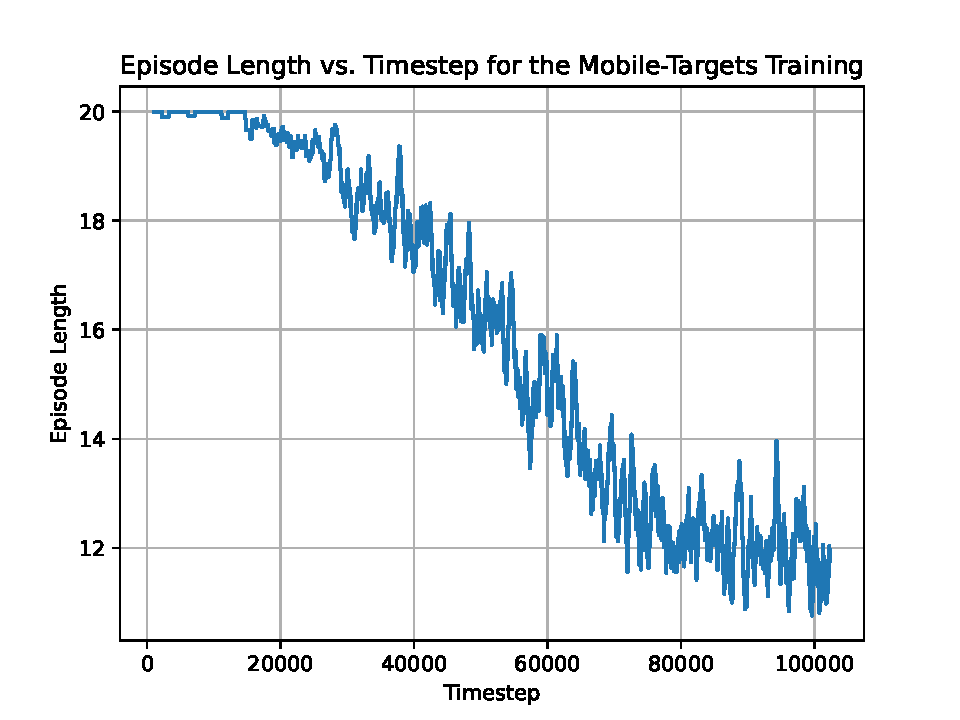
\includegraphics[width=0.8\textwidth]{episode-lengths-mobile}
        \caption{\gls{rl} episode length convergence during the
        mobile-targets training.}
        \label{fig:episode-lengths-mobile}
\end{figure}

\subsection{\textsc{rl} model performance}

In order to verify the advantages of an \gls{rl}-trained drone
in the target visitation mission, we have compared it with
two other baseline agents.

The first agent is a drone that completes the same mission 
while moving completely randomly. 
In other words, the probability of taking each of the 
nine available actions is the same.
The second agent moves in a zig-zag manner, as shown
in \cref{fig:zigzag}.
If this zig-zag agent does not visit all the targets the first time
round, it continues from the final cell and follows the same
path as it came but in reverse.
This overall pattern may start from the beginning (cell 1) or 
the end (cell 25).
We have included both variants, named Zigzag1 and Zigzag2
respectively, to make the comparison comprehensive.

\begin{figure}[!t]
	\centering
	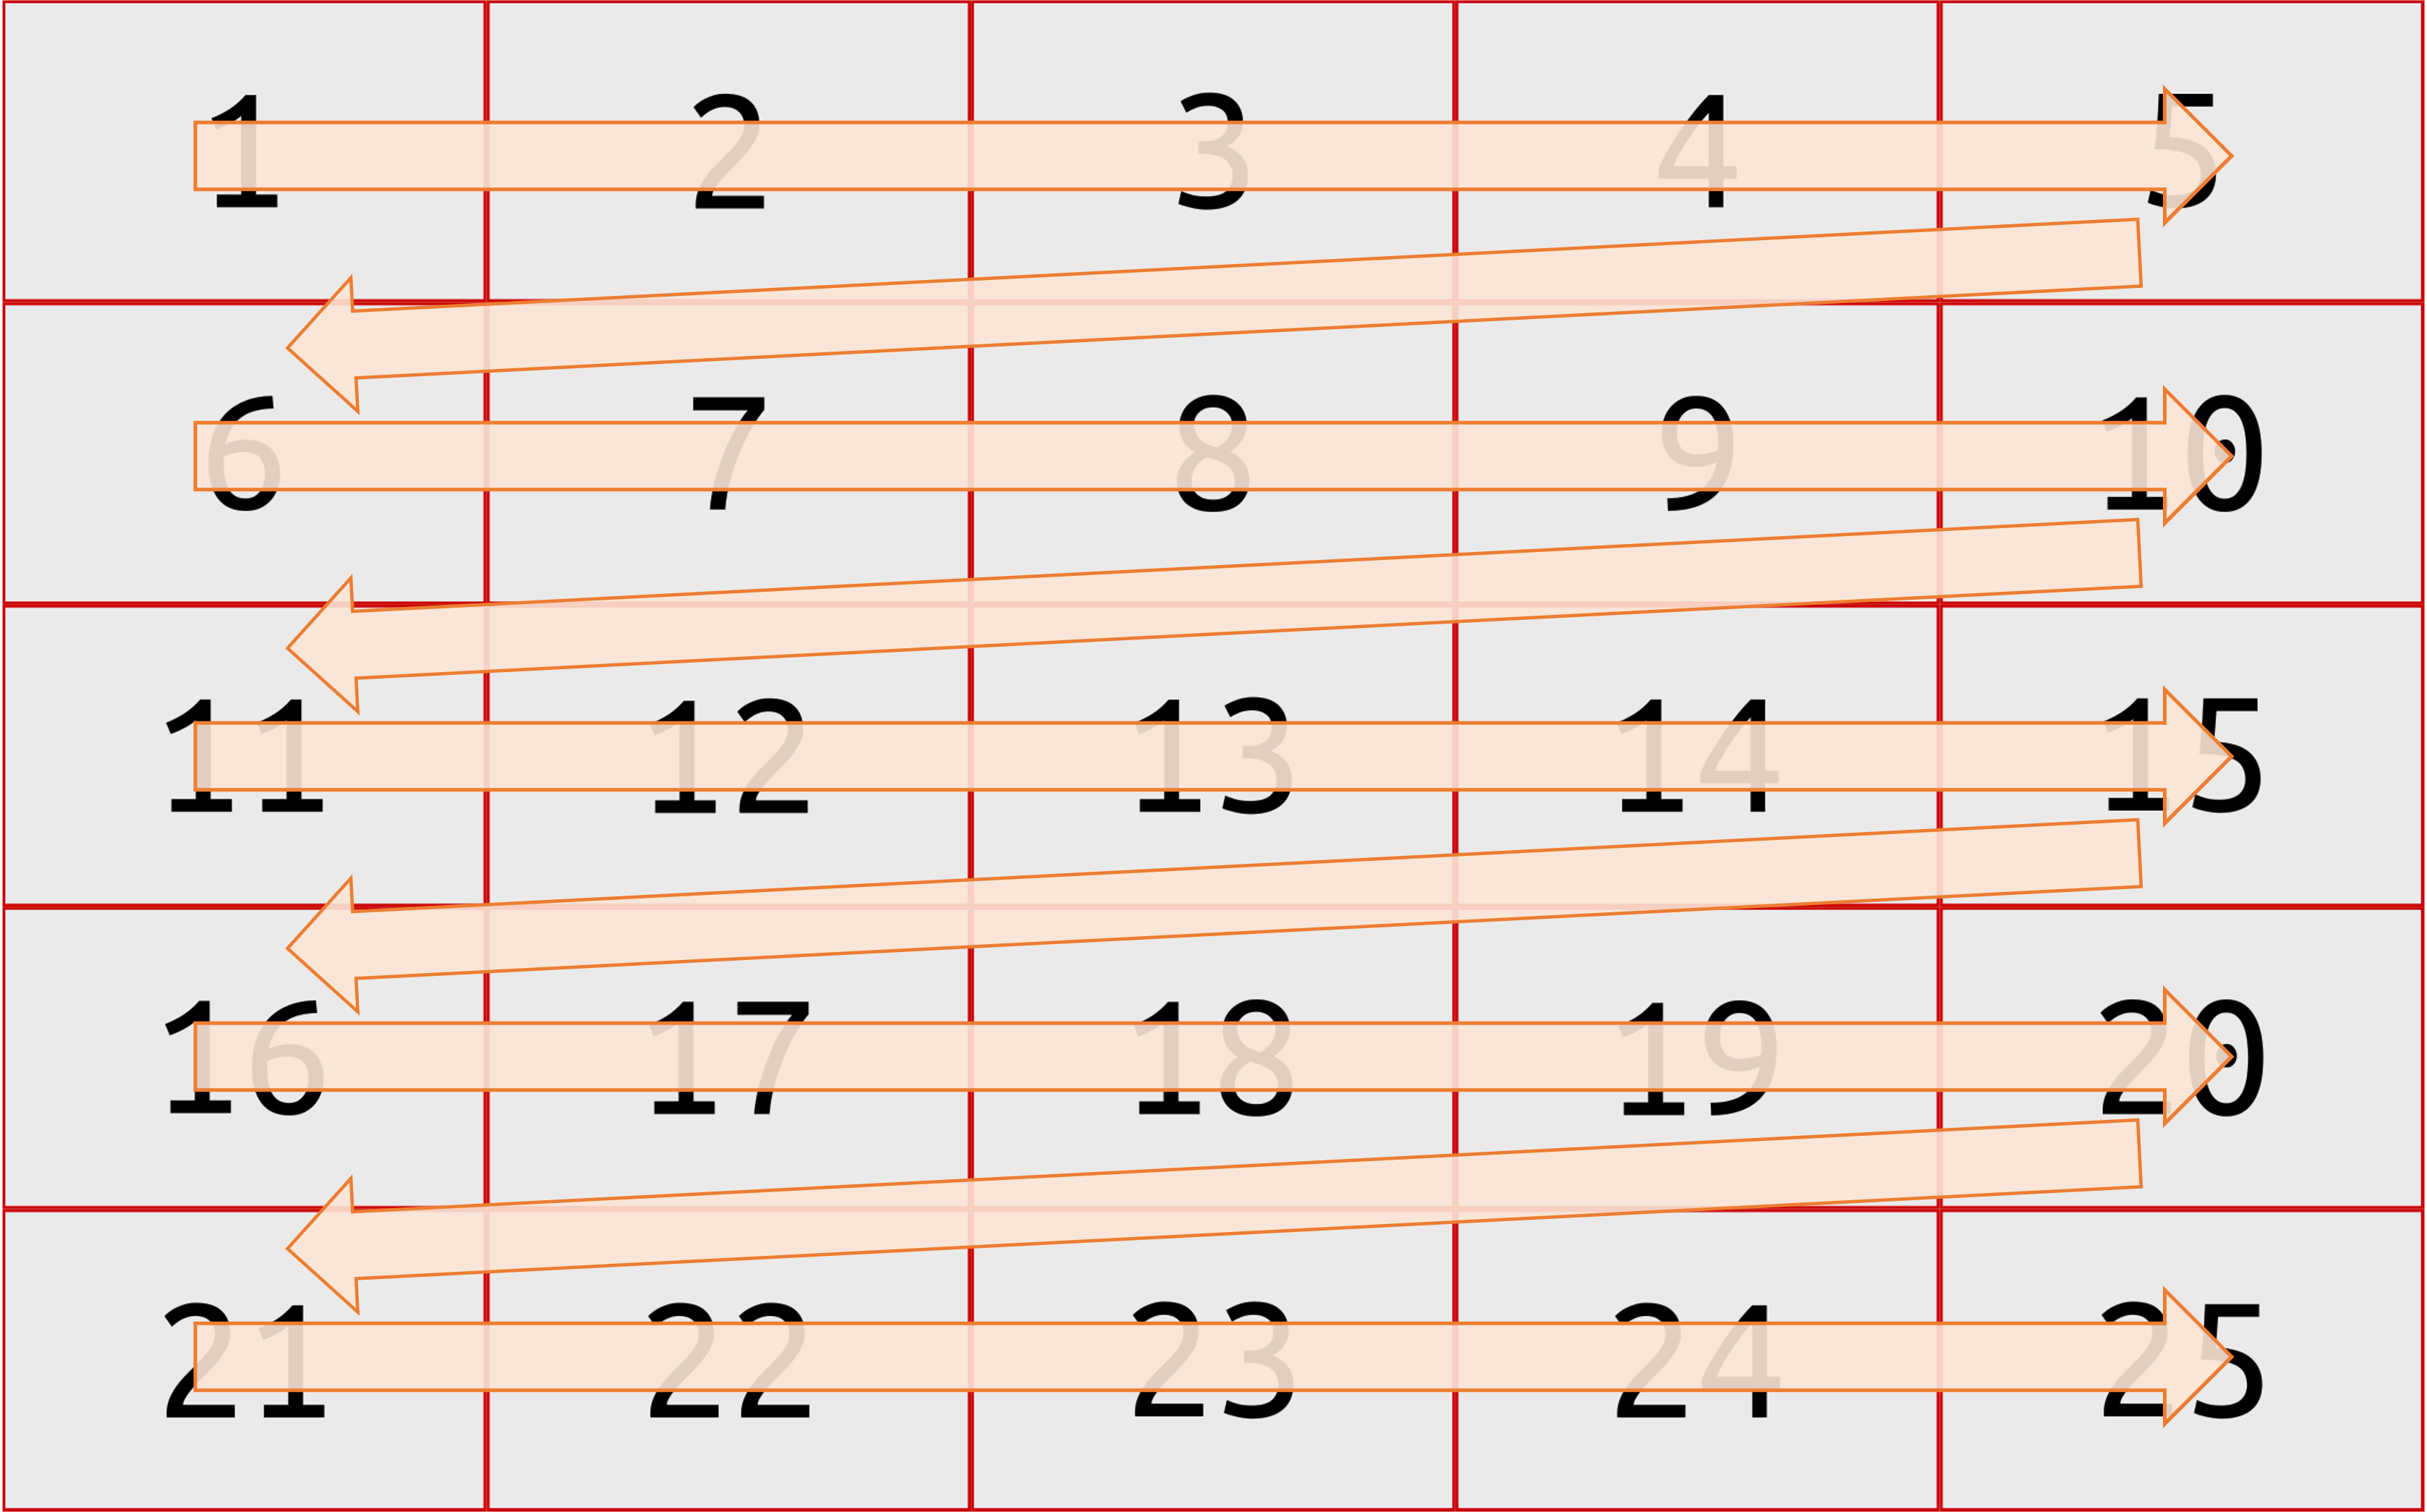
\includegraphics[width=0.8\textwidth]{zigzag}
	\caption{The directions of the drone moving zig-zag
		across the grid according to zigzag-1.
                zigzag-2 begins from cell 25.}
	\label{fig:zigzag}
\end{figure}

To make the comparison objective, 
each of the nine actions executed by random, zig-zag
or \gls{rl} techniques is treated the same way regardless 
of the fluctuations that may arise in the 
distance travelled and speed during
the simulation.
In other words, the distance travelled does not depend
on the technique used but only 
the type of action taken. 
The distances are listed in \cref{tab:distances}.

\begin{table}[tbp]
\caption{The distances travelled by each action based on
    the grid 25x40m\textsuperscript{2} shown in 
    Fig.~\ref{fig:grid}.}
\label{tab:distances}
\centering
\begin{tabular}{p{3.4in} c}
\toprule
Movement directions & Distances, $d$ (m) \\
\midrule
\raggedright Forward-left, forward-right, 
backward-left, backward-right & 9.434 \\
Forward, backward & 5.000 \\
Right, left & 8.000 \\
Starting cell to edge cell e.g. 13\textrightarrow 1 (for zigzag) & 18.868 \\
\raggedright Long diagonal e.g. 5\textrightarrow 6 (for zigzag) & 32.388 \\
\bottomrule
\end{tabular}
\end{table}

On the other hand, the speed is constant for all actions. 
The constant values of speed along with processing time,
and power consumed during movements and hovering
are presented
in \cref{tab:assumptions}
and they are used in the calculations.
Furthermore, since the performance of the agent,
especially the random one, can vary widely and
the positions of the targets are different in each episode, 
10 trials are carried out for each technique and
the average time is taken.

\begin{table}[tbp]
\caption{The values assumed to be constant throughout the
mission.}
\label{tab:assumptions}
\centering
\begin{tabular}{l c c}
\toprule
Parameter & Symbol & Value \\
\midrule
Speed & $v$ & 5 m/s \\
Processing time & $t_{\text{process}}$ & 1 s \\
Hovering time & $t_{\text{hover}}$ & 2 s \\
Power for moving & $P_{\text{move}}$ & 20 W \\
Power for hovering & $P_{\text{hover}}$ & 10 W \\
\bottomrule
\end{tabular}
\end{table}

\Cref{eq:move-time} shows the formula used to
calculate the time taken for a moving action and
\cref{eq:hover-time} for a hovering one.
For the energy, moving actions' consumptions are calculated
by \cref{eq:move-energy} while a hovering one by
\cref{eq:hover-energy}.
\begin{align}
t_{\text{move,tot}} &= 
\frac{d}{v} + t_{\text{process}}
	\label{eq:move-time}
        \\
t_{\text{hover,tot}} &= 
t_{\text{hover}} + t_{\text{process}}
	\label{eq:hover-time}
        \\
E_{\text{move,tot}} &= 
\frac{d}{v} \cdot P_{\text{move}} 
+ t_{\text{process}} \cdot P_{\text{hover}}
	\label{eq:move-energy}
        \\
E_{\text{hover,tot}} &= 
\left( t_{\text{hover}} + t_{\text{process}} \right) \cdot P_{\text{hover}}
	\label{eq:hover-energy}
\end{align}

\subsubsection{Fixed-targets mission}

The results for the fixed-targets mission are presented as bar charts in 
\cref{fig:time-plot-fixed} and \cref{fig:energy-plot-fixed}.
Both of the plots indicate that the \gls{rl} agent completed
the mission in the shortest time and least energy, followed
by the Zigzag2 since it started in an area 
where the probability
distribution of the targets is the highest.
In fact, the \gls{rl} agent is about twice as fast and twice
as energy-saving as Zigzag2.

\begin{figure}[tbp]
	\centering
	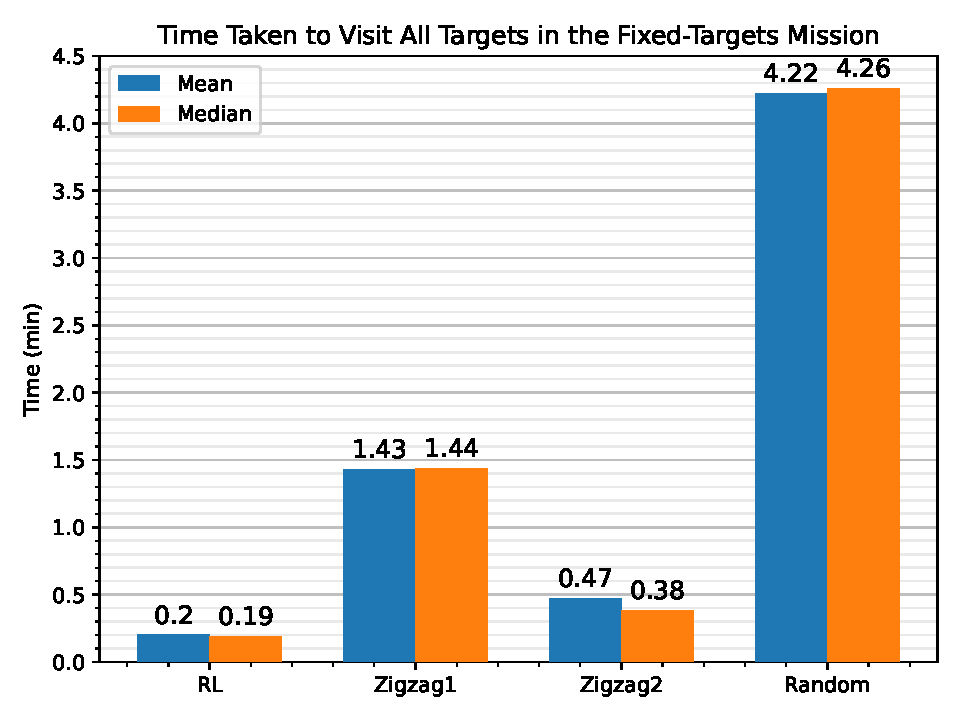
\includegraphics[width=0.8\textwidth]{time-plot-fixed}
	\caption{The time taken by each technique
            to complete the fixed-targets mission showing the mean and
    median.}
        \label{fig:time-plot-fixed}
\end{figure}

\begin{figure}[tbp]
	\centering
	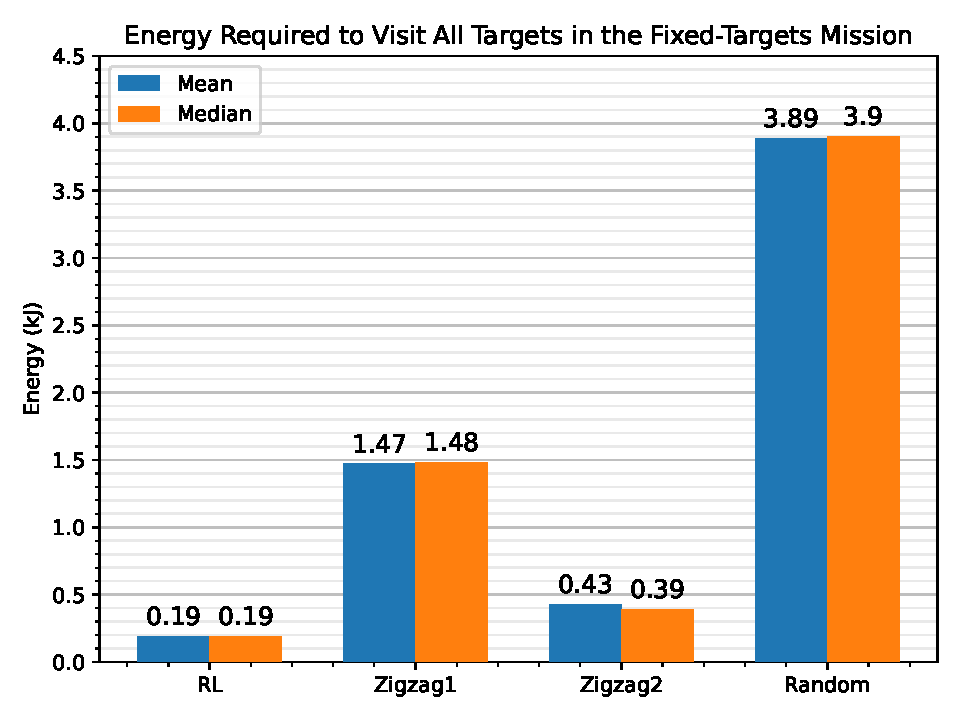
\includegraphics[width=0.8\textwidth]{energy-plot-fixed}
	\caption{The energy consumed by each technique
            to complete the fixed-targets mission showing the mean and
    median.}
        \label{fig:energy-plot-fixed}
\end{figure}

The \gls{rl} performed the best in this environment because
the targets were not placed in a uniform distribution
across the grid,
in which the random agent may have equalled the performance,
neither were they placed deterministically, 
in which case the zig-zag technique with the
right starting point would have won.
Another interesting observation from the comparison is that
the \gls{rl} agent did not execute the hovering action at all
because after so many timesteps choosing to hover and
receiving a reward of -1, it has learnt that it is an
action that is not beneficial in all states.

\subsubsection{Mobile-targets mission}

For the mobile-targets mission, the results for time taken and energy consumed are shown in 
\cref{fig:time-plot-mobile} and \cref{fig:energy-plot-mobile} respectively.
Again, the \gls{rl} agent performed the best, more than two times
faster and more energy-saving than the
second fastest and the second energy-saving agent which is Zigzag2.
Zigzag2 started from cell 25, and by the time it took it to reach
cell 1, the moving targets had already got to their north-west
destination corner and moved within the cell 1 only.

In contrast, Zigzag1 started from cell 1 and in the first round it
missed the moving targets as they moved to the cells already covered
by the Zigzag1 agent.
Therefore, it had to restart scanning in reverse before it
covered all the targets making it much slower than Zigzag2.
As expected, the random agent performed the worst as it did not follow
any particular strategy to visit the targets. It only relied on
chances.

\begin{figure}[tbp]
	\centering
	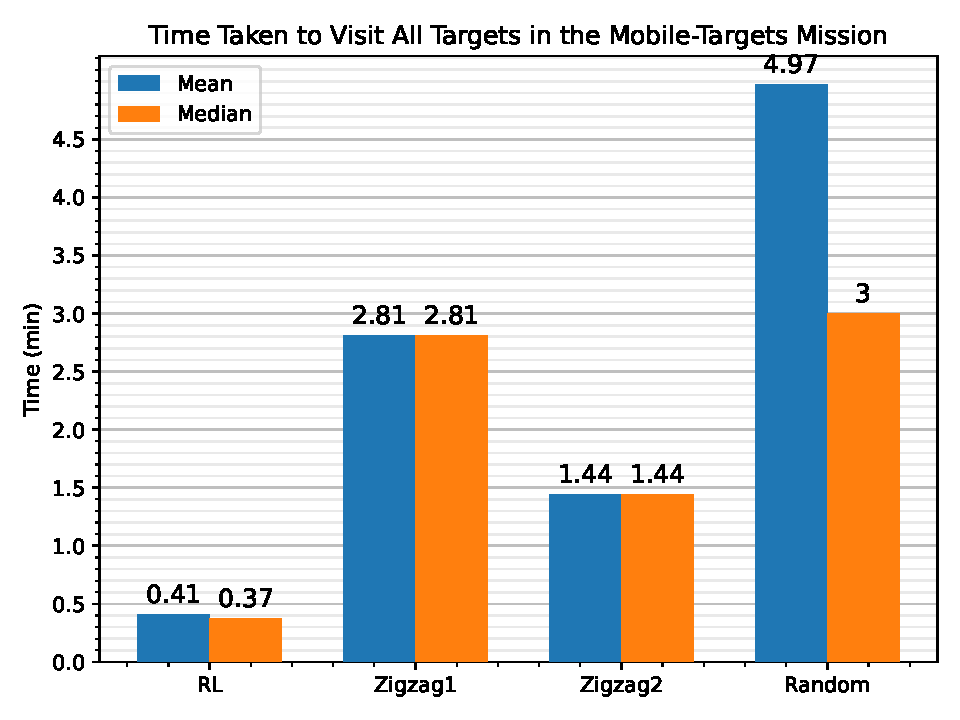
\includegraphics[width=0.8\textwidth]{time-plot-mobile}
	\caption{The time taken by each technique
        to complete the mobile-targets mission showing the mean and
    median.}
        \label{fig:time-plot-mobile}
\end{figure}

\begin{figure}[tbp]
	\centering
	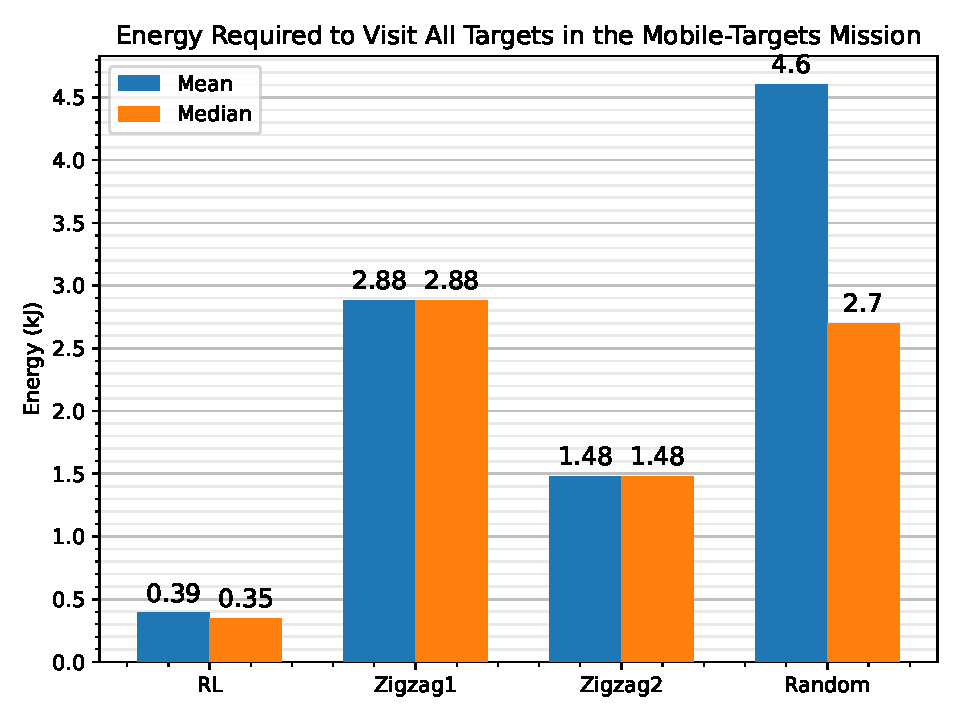
\includegraphics[width=0.8\textwidth]{energy-plot-mobile}
	\caption{The energy consumed by each technique
        to complete the mobile-targets mission showing the mean and
    median.}
        \label{fig:energy-plot-mobile}
\end{figure}

\subsection{Drone's height}

For certain scenarios, it is required that the agent performs the
mission in an environment that is scaled down from that used in the
training.
Such scenario occurred in this project for the full integration
testing, in which we had to print the \textsc{qr} codes in A4-sized papers due
to our limited resources instead of the 0.7x0.7m material used in the
training environment.
To detect these smaller targets, we had to decrease the height of the
drone.
In turn, the cell size also needed to be reduced so that the agent at
this new lower height can see the entire cell, and we have used
\cref{fig:h-alt} to figure out this size.

\begin{figure}[tbp]
	\centering
	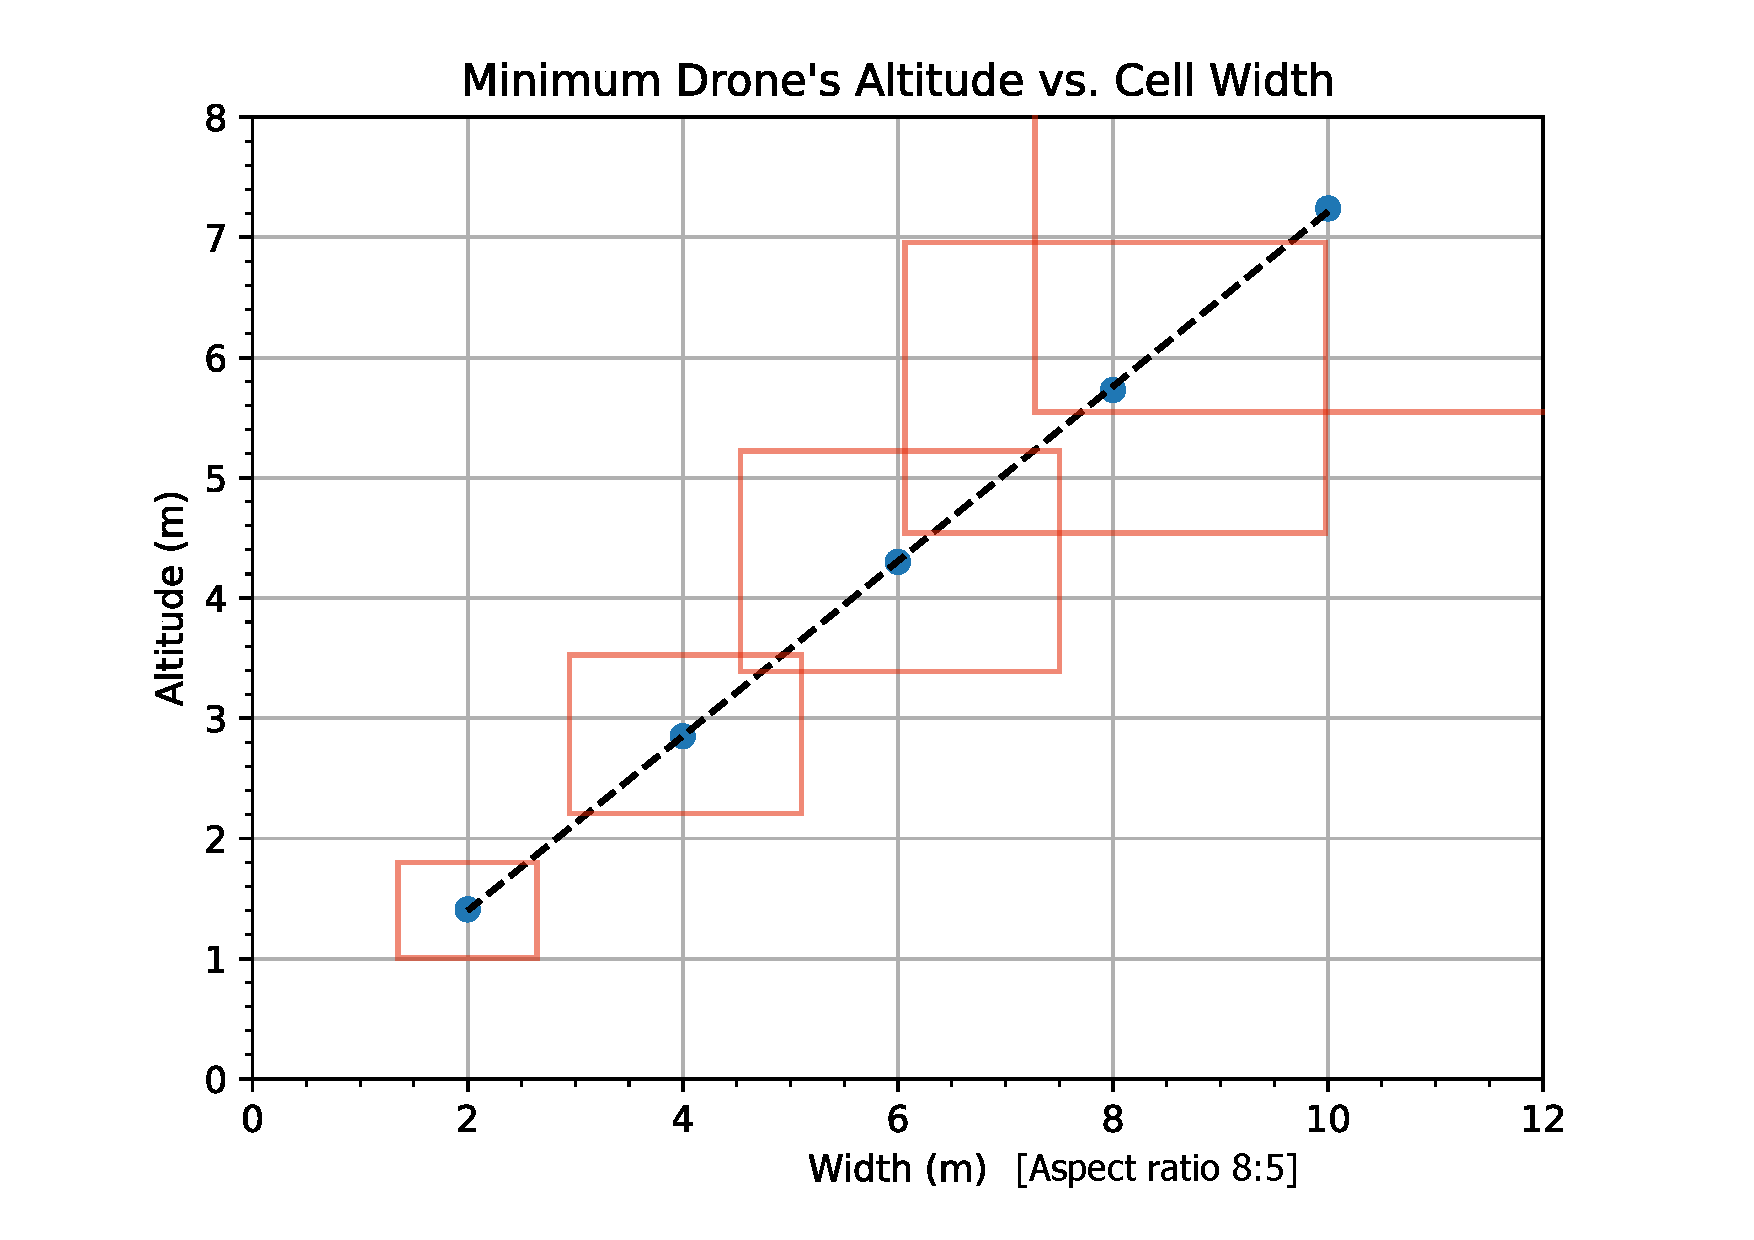
\includegraphics[width=0.8\textwidth]{h-alt}
	\caption{The minimum height that the drone needs to fly at to
        fully cover the cell underneath with the given width.  
        The aspect ratio of each cell is eight-to-five.}
	\label{fig:h-alt}
\end{figure}

To obtain the graph in~\cref{fig:h-alt}, we have flown the drone in
the simulation environment at multiple heights, and below, the ground
was replaced with cells of different sizes as shown
in~\cref{fig:h-alt-ground}.
We then recorded which maximum cell size was the drone able to capture
using its camera and fit a linear regression line through these
points. 

\begin{figure}[tbp]
	\centering
	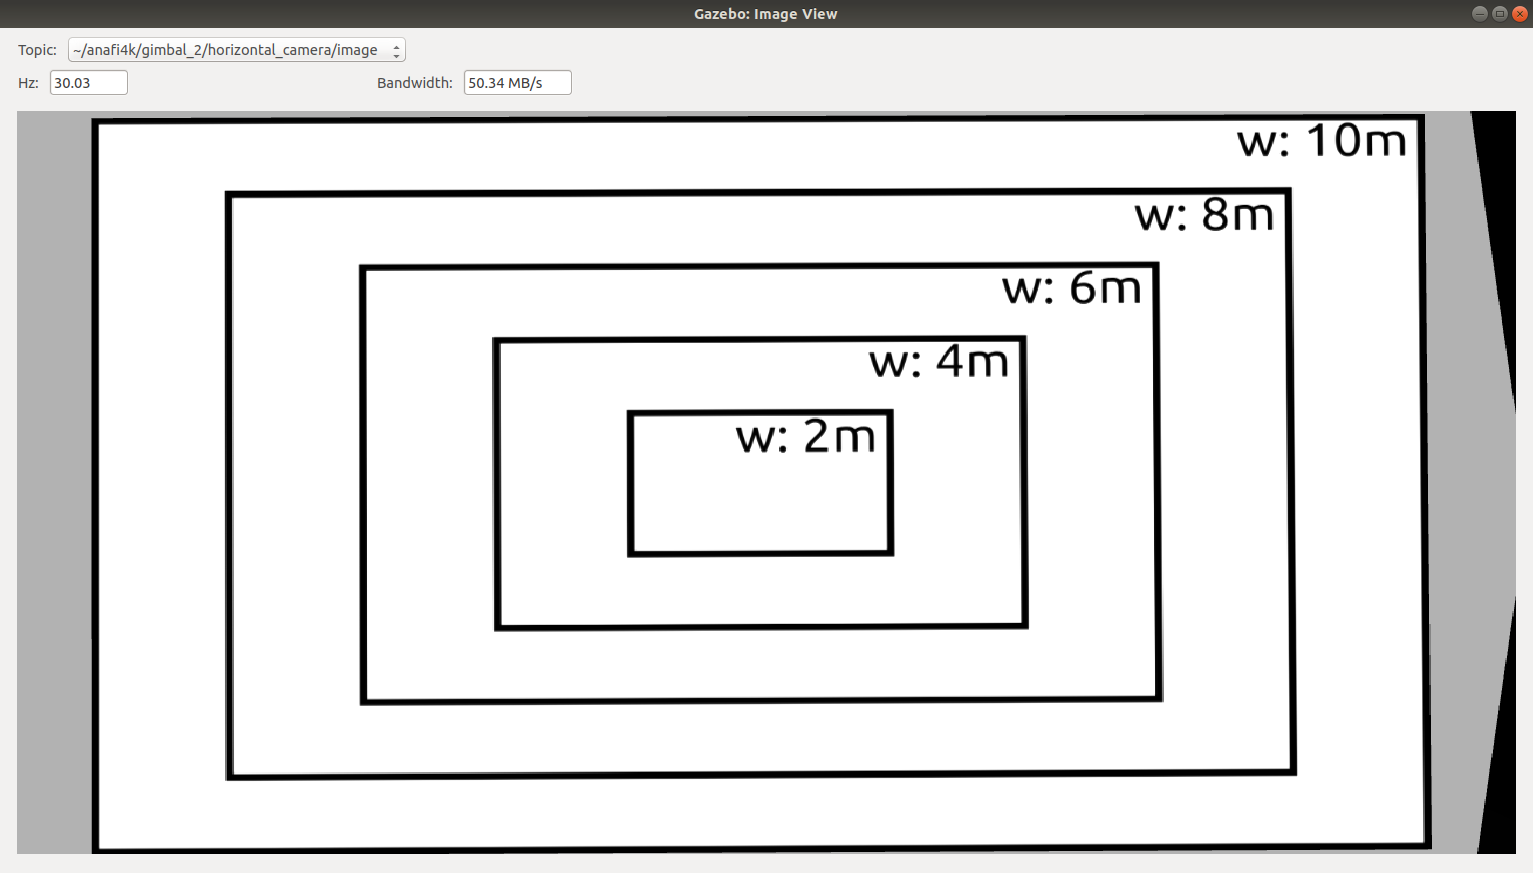
\includegraphics[width=0.8\textwidth]{h-alt-ground}
	\caption{Cells of varying widths as seen by the drone's camera.
        The aspect ratio of all cells is the same which is
        eight-to-five.}
	\label{fig:h-alt-ground}
\end{figure}

\subsection{User interface}

\lipsum[1]


\end{document}
